\documentclass[11pt]{book} % 11pt font
\usepackage{amsmath}
\usepackage{amsfonts}
\usepackage{bm}
\usepackage{graphicx}
\usepackage{mathtools}
\usepackage{physics}
\usepackage{pgfplots}
\usepackage{accents}
\usepackage{geometry}
\usepackage{caption}

% my custom commands
% ------------------
% note command
\newcommand{\note}[1]{\textsf{\textcolor{red}{#1}}}
% multi-line comment command
\newcommand{\comment}[1]{}
\newcommand{\del}{\bm{\nabla}}
\newcommand{\partder}[2]{\frac{\partial #1}{\partial #2}}
\newcommand{\compcon}{+\text{c.c}}
\graphicspath{{./images}}


% -------------------------
% BEGINNING OF THE DOCUMENT
% -------------------------
\begin{document}

\chapter{Fall Term, Hailin Wang}
\section{Overview}
The start of the course will mainly focus on two level states (5-6 weeks) and then we move on to 3 level states and the mechanical effects of light. \\
This course will focus on how does light interact with matter.\\
This interaction can be done in terms of semi-classical physics, where we have classical light and quantum mechanical matter, or a pure quantum approach which treats both light and matter quantum mechanically.\\

\section{Two-Level quantum systems (aka the Rabi problem)}
In a simple system we have discrete atomic energy levels and a single opticla mode of light:
\begin{align*}
	\frac{1}{2} E_0 e^{-i\omega t} + \text{c.c.}
\end{align*}
But this discrete set of atomic energy levels is still too complicated since there are an infinite number of states for the atom. In order to further simplify things we limit ourselves to two-level systems where our atom can be in state $\ket{1}$ or $\ket{2}$.\\
If we have transition energy between the two states that has a corresponding energy $\omega_0$ and an optical field at $\omega$, we then have a detuning $\delta = \omega_0-\omega$, resonance when $\omega=\omega_0$, and near resonance when $\omega\approx\omega_0$.\\
When we are near resonance we ignore all off-resonant interactions.\\
We now come up with our Hamiltonian (after which we will try to solve the Schroedinger equation).
\begin{align*}
	H &= H_0 + V \\
	H_0 &= \begin{pmatrix} E_1 & 0 \\ 0 & E_2\end{pmatrix} \\
	H_0 &= \hbar\begin{pmatrix} \omega_1 & 0 \\ 0 & \omega_2\end{pmatrix}
\end{align*}
We now use the fact that $\omega_1 - \omega_2 = \omega_0$, so we rewrite this as:
\begin{align*}
	H_0 &= \frac{\hbar}{2}\begin{pmatrix} -\omega_0 & 0 \\ 0 & \omega_0\end{pmatrix} \\
	H_0 &= -\frac{\hbar\omega_0}{2}\begin{pmatrix} 1 & 0 \\ 0 & -1\end{pmatrix}
\end{align*}
Since atoms are neutral, if our wavelength is much larger than the bohr radius we can model this with a dipole interaction.\\
Our dipole potential is:
\begin{align*}
	V &= -\bm{\mu}\cdot\bm{E} \\
	\bm{\mu} &= -e\bm{r} \\
	\bm{E} &= |E_0| \cos(\omega t-\phi)\hat{\epsilon}
\end{align*}
We could in principle add a quadrapole, magnetic dipole interaction, etc.\\
If we have our field point allong the z axis we can write:
\begin{align*}
	V_{12} &= \bra{1} V\ket{2} \\
	V_{12} &= e Z_{12} |E_0| \cos(\omega t -\phi) \\
	V_{11} &= \bra{1} V\ket{1} \\
	V_{11} &= e Z_{11} |E_0| \cos(\omega t -\phi) \\
	V_{22} &= \bra{2} V\ket{2} \\
	V_{22} &= e Z_{22} |E_0| \cos(\omega t -\phi)
\end{align*}
But we know $Z_{11} = Z_{22} = 0$ by symettry (though this may not hold inside some crystals). \\
Therefore we can then write:
\begin{align*}
	V &= \begin{pmatrix} V_{12} & 0 \\ 0 & V_{21} \end{pmatrix}
\end{align*}
We define $\Omega_0$ (the Rabi frequency).
\begin{align*}
	\Omega_0 &= -\frac{\mu_{12} E_0}{\hbar}
\end{align*}
By convention we choose the phase of $\mu_{12} = -e Z_{12}$ to make it real. Therefore we have:
\begin{align*}
	V_{12} &= \hbar |\Omega_0| \cos (\omega t -\phi) \\
	V &= \hbar |\Omega_0| \cos (\omega t - \phi)\begin{pmatrix}
		0 & 1 \\
		1 & 0
      \end{pmatrix}
\end{align*}
In terms o the Pauli matricies we then have:
\begin{align*}
	H_0 &= -\frac{\hbar\omega_0}{2} \sigma_z \\
	V &= \hbar |\Omega_0|\cos(\omega t - \phi) \sigma_x \\
	H &= -\frac{\hbar\omega_0}{2} \sigma_z + \hbar |\Omega_0|\cos(\omega t - \phi) \sigma_x
\end{align*}
The key parameters in question for this hamiltonian are the detuning, $\delta=\omega_0-\omega$ and the Rabi frequency $\Omega_0$. \\
\subsection{Interaction representation and rotating wave approximation}
In the Schroedinger representation:
\begin{align*}
	\ket{\psi(t)} &= \sum_n c_n(t) \ket{n} \\
	i\hbar \partial_t \ket{\psi(t)} &= H\ket{\phi(t)}
\end{align*}
If we assume that we have a phase of zero, so $\Omega_0$ is real:
\begin{align*}
	i\hbar \partial_t \begin{pmatrix}c_1 \\ c_2\end{pmatrix} &= H \begin{pmatrix}c_1 \\ c_2\end{pmatrix} \\
	i\hbar \partial_t \begin{pmatrix}c_1 \\ c_2\end{pmatrix} &= \hbar \begin{pmatrix} -\frac{\omega_0}{2} & \Omega_0 \cos\omega t \\ \Omega_0\cos\omega t & \frac{\omega_0}{2}\end{pmatrix} \begin{pmatrix}c_1 \\ c_2\end{pmatrix} \\
	\dot{c_1} &= i \frac{\omega_0}{2} c_1 - i\Omega_0\cos\omega t c_2 \\
	\dot{c_2} &= i \frac{\omega_0}{2} c_2 - i\Omega_0\cos\omega t c_1
\end{align*}
If $\Omega_0 = 0$ we just get free evolution, so we only have phase evolution for both terms. \\
In the interaction representation we put the evolution from $H_0$ into the states, so:
\begin{align*}
	\ket{\psi(t)} &= \sum_n \bar{c_n}(t) e^{-i \omega_n t} \ket{n}
\end{align*}
So our equation of motion becomes:
\begin{align*}
	i \hbar \partial_t \begin{pmatrix}\bar{c_1} \\ \bar{c_2} \end{pmatrix} &= V_I \begin{pmatrix}\bar{c_1} \\ \bar{c_2}\end{pmatrix}
\end{align*}
We know from our definitions for the interaction picture:
\begin{align*}
	\bar{c_n} &= c_n e^{i\omega_n t} \\
	\dot{\bar{c_n}} &= \dot{c_n} e^{i\omega_n t} + i\omega_n c_n e^{i\omega_n t} \\
	\dot{\bar{c_1}} &= \left(i \frac{\omega_0}{2} c_1 - i\Omega_0\cos\omega t c_2 \right) e^{-i\frac{\omega_0}{2} t} -\frac{i\omega_0}{2}c_1 e^{-i\frac{\omega_0}{2} t} \\
	\dot{\bar{c_1}} &= - i\Omega_0\cos\omega t c_2  e^{-i\frac{\omega_0}{2} t} \\
	\dot{\bar{c_1}} &= -i\Omega_0\cos\omega t \bar{c_2}e^{-i\omega_0 t} \\
	\dot{\bar{c_2}} &= -i\Omega_0\cos\omega t \bar{c_1} e^{i\omega_0 t}
\end{align*}
Therefore:
\begin{align*}
	V_I &= \hbar \Omega_0 \cos\omega t \begin{pmatrix}
		0 & e^{-i\omega_0 t} \\
		e^{i\omega_0 t} & 0
		\end{pmatrix}
\end{align*}
So working in the interaction picture here has simply removed the diagonal part of the Hamiltonian. \\
We now seek to solve our equations for our amplitudes here, we start be rewriting cosine in terms of complex exponentials:
\begin{align*}
	\dot{\bar{c_1}} &= -i\frac{\Omega_0}{2}\left(e^{i\omega t} + e^{-i\omega t}\right)e^{-i\omega_0 t}\bar{c_2} \\
	\dot{\bar{c_1}} &= -i\frac{\Omega_0}{2}\left(e^{i(\omega-\omega_0) t} + e^{-i(\omega+\omega_0) t}\right)\bar{c_2} \\
	\dot{\bar{c_2}} &= -i\frac{\Omega_0}{2}\left(e^{i\omega t} + e^{-i\omega t}\right)e^{i\omega_0 t}\bar{c_1} \\
	\dot{\bar{c_2}} &= -i\frac{\Omega_0}{2}\left(e^{i(\omega_0-\omega) t} + e^{i(\omega + \omega_0)t}\right)\bar{c_1}
\end{align*}
We now break this into a perurbation series:
\begin{align*}
	\bar{c_n} &= \bar{c}_n^{(0)} + \bar{c}_n^{(1)} +\bar{c}_n^{(2)} + \ldots \\
	\bar{c}_n^{(m)} &\propto E_0^m 
\end{align*}
If we start in state 1:
\begin{align*}
	\dot{\bar{c}_1^{(1)}} &\propto \bar{c}_2^{(0)} = 0 \\
	\dot{\bar{c}_2^{(1)}} &=-i\frac{\Omega_0}{2}\left(e^{i(\omega_0 - \omega) t} + e^{i(\omega_0 + \omega)t}\right)
\end{align*}
So we have after integration:
\begin{align*}
	\bar{c}_2^{(1)}(t) &= -i\frac{\Omega_0}{2} \left[ \frac{e^{i\omega_0-\omega)t} -1 }{i(\omega_0-\omega} + \frac{e^{i(\omega_0 + \omega) t} - 1}{i(\omega_0 + \omega)}\right]
\end{align*}
If we are near resonance the second term is much smaller, and $\Omega_0 << \omega_0$ we use the rotating wave approximation:
\begin{align*}
	\bar{c}_2^{(1)}(t) &= -i\frac{\Omega_0}{2}\frac{e^{i\omega_0-\omega)t} -1 }{i(\omega_0-\omega} 
\end{align*}
Which equivalently in the hamiltonian has:
\begin{align*}
	V_I &= \hbar \frac{\Omega_0}{2} \begin{pmatrix}
		0 & e^{-i\delta t} \\
		e^{i\delta t} & 0
		\end{pmatrix}
\end{align*}
If we generalize we have (with some phase on $\Omega_0$):
\begin{align*}
	V_I &= \frac{\hbar }{2} \begin{pmatrix}
		0 & \Omega_0^*e^{-i\delta t} \\
		\Omega_0e^{i\delta t} & 0
		\end{pmatrix}
\end{align*}
\subsection{The exact solution of the Rabi problem (with rotating wave approximation)}
Next class we will solve this, we will get $\pi$ pulses, Rabi oscilations, etc.

\subsection{Review of last class}
In the interaction between a 2 level system and an optical field, we have an interaction potential $V= -\bm{\mu}\cdot\bm{E}$. We worked in the interaction picture, which removed the free interaction dependance from our states (at the cost of making our interaction potential slightly more complicated). We then made the rotating wave approximation, where we drop all counter rotating terms from the interaction potantial.
\subsection{Rabi Problem and the exact solution}
We define the spin-flip opertors:
\begin{align*}
	\sigma_+ &= \begin{pmatrix}
		0 & 0 \\
		1 & 0
	     \end{pmatrix} \\
	\sigma_- &= \begin{pmatrix}
		0 & 1 \\
		0 & 0
	     \end{pmatrix}
\end{align*}
So we can then write our interaction potential as:
\begin{align*}
	V_I &= \frac{\hbar}{2} \Omega_0 e^{i\delta t} \sigma_+ + \text{h.c.}
\end{align*}
And we know:
\begin{align*}
	\sigma_+ \ket{1} &= \ket{2} \\
	\sigma_+ \ket{2} &= 0 \\
	\sigma_- \ket{2} &= \ket{1} \\
	\sigma_- \ket{1} &= 0
\end{align*}
We now try to solve our equation for some special cases. If we pick exact resonance, so our detuning is zero, and a constant $\Omega_0$ we have:
\begin{align*}
	\dot{\bar{c}}_1 &= -\frac{i\Omega_0}{2} \bar{c}_2 \\
	\ddot{\bar{c}}_1 &= -\frac{\Omega_0^2}{4} \bar{c}_1 \\
	\dot{\bar{c}}_2 &= -\frac{i\Omega_0}{2} \bar{c}_1 \\
	\ddot{\bar{c}}_2 &= -\frac{\Omega_0^2}{4} \bar{c}_2
\end{align*}
This emits solutions in the form of sines and cosines. If we assume the population starts in state $\ket{1}$ we have:
\begin{align*}
	\bar{c}_1 &= \cos\left(\frac{\Omega_0}{2} t\right) \\
	\bar{c}_2 &= -i\sin\left(\frac{\Omega_0}{2} t\right)
\end{align*}
Since the probability is the square of the amplitude we have oscilations between the states with frequency $\Omega_0$.

If instead we have a variable $\Omega_0$ but exact resonance we have a more difficult problem to solve. In order to solve this we define:
\begin{align*}
	\bar{c}_\pm &= \bar{c}_1 \pm \bar{c}_2 \\
	\dot{\bar{c}}_+ &= -i\frac{\Omega_0}{2} \bar{c}_+ \\
	\dot{\bar{c}}_- &= i\frac{\Omega_0}{2} \bar{c}_-
\end{align*}
So our solutions are:
\begin{align*}
	\bar{c}_+(t) &= \bar{c}_+(0) e^{-i\int_0^t dt' \frac{\Omega_0}{2}} \\
	\bar{c}_-(t) &= \bar{c}_-(0) e^{i\int_0^t dt' \frac{\Omega_0}{2}}
\end{align*}
We now define the pulse area:
\begin{align*}
	A(t) &= \int_0^t dt' \Omega_0(t)
\end{align*}
So:
\begin{align*}
	\bar{c}_+(t) &= \bar{c}_+(0) e^{-\frac{i}{2}A(t)} \\
	\bar{c}_-(t) &= \bar{c}_-(0) e^{\frac{i}{2}A(t)}
\end{align*}
So then:
\begin{align*}
	\begin{pmatrix}
		\bar{c}_1(t) \\
		\bar{c}_2(t)
	\end{pmatrix} &= \begin{pmatrix}
	\cos\frac{A}{2} & -i\sin\frac{A}{2} \\
	-i\sin\frac{A}{2} & \cos\frac{A}{2}
		  \end{pmatrix}
		  \begin{pmatrix}
			  \bar{c}_1(0) \\
			  \bar{c}_2(0)
    \end{pmatrix}
\end{align*}
Which corresponds to oscilatory behavior, but with respect to the pulse area rather than time.\\
We can therefore talk about a $\pi$ pulse, which has a total pulse area of $\pi$, aka $\lim_{t\to\infty} A(t) = \pi$. This will cause the population to swap and gain a phase of $-i$.\\
Similarly a $2\pi$ pulse will only add an overall $-1$ phase to both $\bar{c}_1$. This is a Berry phase. \\
We finally consider a non-zero detuning with a constant Rabi frequency:
\begin{align*}
	\ddot{\bar{c}}_1 &= -i\delta\dot{\bar{c}}_1  - \frac{\Omega_0^2}{4} \bar{c}_1 \\
\ddot{\bar{c}}_2 &= i\delta\dot{\bar{c}}_2  - \frac{\Omega_0^2}{4} \bar{c}_2
\end{align*}
These emit complex exponential solutions, our solution is therefore:
\begin{align*}
	\Omega &= \sqrt{\Omega_0^2 + \delta^2} \\
	\gamma &= -\frac{i\delta}{2} \pm i\frac{\Omega}{2}
	\bar{c}_1 &= \bar{c}_1(0) e^{\gamma t}
\end{align*}
$\Omega$ is the generalize Rabi frequency. Our solution is therefore:
\begin{align*}
	\bar{c}_1 &= e^{i\frac{\delta}{2} t} \left[ B_1 \cos \frac{\Omega t}{2} + B_2 \sin \frac{\Omega t}{2}\right] \\
	\bar{c}_2 &= \frac{\dot{\bar{c}}_1}{-i\frac{\Omega_0}{2} e^{-i\frac{\delta}{2} t}} \\
	\bar{c}_2 &= e^{i\frac{\delta}{2} t} \left[ B_1 \sin \frac{\Omega t}{2} + B_2 \cos \frac{\Omega t}{2}\right]
\end{align*}
If we start with our population in state 1, then:
\begin{align*}
	|\bar{c}_2(t)|^2 &= \left(\frac{\Omega_0}{\Omega}\right)^2 \sin \frac{\Omega t}{2} \\
\end{align*}
If we return to the Schroedinger represntation, we see that the energy levels appear to be shifting due to this applied optical field. This is known as the optical Stark shift.\\
So far we have assumed this is a perfect system, if we assume that we can actually decay out of the system, we have:
\begin{align*}
	\partial_t |\bar{c}_1|^2 &= -\gamma_2|\bar{c}_1|^2 \\
	\partial_t |\bar{c}_2|^2 &= -\gamma_2|\bar{c}_2|^2
\end{align*}
This corresponds to a decay term that is half the given rate in the amplitude. We can seey this bay taking the onsatz that it is half and quckly see this is true:
\begin{align*}
	\partial_t \bar{c}_1 &= -\frac{\gamma_1}{2} \bar{c}_1 \\
	\partial_t |\bar{c}_1|^2 &= \dot{\bar{c}}_1\bar{c}_1^* + \bar{c}_1 \dot{\bar{c}}_1^* \\
	\partial_t |\bar{c}_1|^2 &= \frac{\gamma}{2}\bar{c}_1\bar{c}_1^* + \frac{\gamma}{2}\bar{c}_1 \bar{c}_1^* \\
	\partial_t |\bar{c}_1|^2 &= \gamma |\bar{c}_1|^2
\end{align*}
\subsection{Field interaction representation/ rotating frame}
In the Schroedinger represntation:
\begin{align*}
	\ket{\psi} &= \sum_n c_n \ket{n} \\
	H\ket{n} &= \hbar\omega_n\ket{n}
\end{align*}
In the interaction represntation
\begin{align*}
	\ket{\psi} &= \sum_n \bar{c}_n e^{-i\omega_n t}\ket{n} \\
\end{align*}
In a two level system:
\begin{align*}
	i\hbar\partial_t \begin{pmatrix}
		\bar{c}_1 \\
		\bar{c}_2 
	\end{pmatrix} &= V_I \begin{pmatrix}
	\bar{c}_1 \\
	\bar{c}_2
		      \end{pmatrix}
	V_I &= \frac{\hbar}{2} \begin{pmatrix}
		0 & \Omega_0^* e^{-i\delta t} \\
		\Omega_0 e^{i\delta t} & 0
			\end{pmatrix}
\end{align*}
In order to work with a time-independant H, we pick a new set of coefficients:
\begin{align*}
	\ket{\psi} \tilde{c}_1 e^{i\frac{\omega}{2} t} \ket{1} + \tilde{c}_2 e^{i\frac{\omega}{2} t}\ket{2}
\end{align*}
So:
\begin{align*}
	\tilde{c}_1 &= \bar{c}_1 e^{i\frac{\delta}{2} t} \\
	\tilde{c}_2 &= \bar{c}_2 e^{-i\frac{\delta}{2} t} \\
	\dot{\tilde{c}}_1 &= i\frac{\delta}{2} \tilde{c}_1 -\frac{i\Omega_0^*}{2} \tilde{c}_2 \\
	\dot{\tilde{c}}_2 &= -i\frac{\delta}{2} \tilde{c}_2 -\frac{i\Omega_0}{2} \tilde{c}_1
\end{align*}
So our Hamiltonian becomes:
\begin{align*}
	i\hbar \partial_t \begin{pmatrix}
		\tilde{c}_1 \\
		\tilde{c}_2 
	\end{pmatrix} &= \tilde{H} \begin{pmatrix}
\tilde{c}_1 \\
\tilde{c}_2
			    \end{pmatrix} \\
	\tilde{H} &= -\frac{\hbar\delta}{2} \begin{pmatrix}
		1 & 0 \\
		0 & -1
	\end{pmatrix} + \frac{\hbar}{2} \begin{pmatrix}
		0 & \Omega_0^* \\
		\Omega_0 & 0
				 \end{pmatrix}
\end{align*}
This looks like a frequency difference between the two states, but with a D.C. coupling between the states. This is different from the interaction picture where we remove the frequency difference but keep an ac transition, or the Schroedinger picture where we have a frequncy difference and AC coupling.
\subsection{Next week}
Unitary transformations, solving $\tilde{H}$ to find it's eigenstates (in the field interaction representation). These states are the semi-classical dressed states. This also relates to optical stark effects and optical stark splitting.

\subsection{Unitary Transformations}
We change basis by using the unitary transform:
\begin{align*}
	\ket{\psi'} &= U\ket{\psi}
\end{align*}
And we want our new Hamiltonian $H'$ s.t.:
\begin{align*}
	i\hbar \partial_t \ket{\psi'} &= H'\ket{\psi'}
\end{align*}
So starting from our untransformed term:
\begin{align*}
	i\hbar \partial_t \ket{\psi} &= H\ket{\psi} \\
	i\hbar \partial_t U^\dagger\ket{\psi'} &= HU^\dagger\ket{\psi'}\\
	Ui\hbar \partial_t U^\dagger\ket{\psi'} &= UHU^\dagger\ket{\psi'}\\
	Ui\hbar \left( \dot{U}^\dagger\ket{\psi'} + U^\dagger\partial_t \ket{\psi'}\right) &= UHU^\dagger\ket{\psi'}\\
	i\hbar \partial_t \ket{\psi'} &= UHU^\dagger\ket{\psi'} - i\hbar U\dot{U}^\dagger\ket{\psi'} \\
	H' &= UHU^\dagger -i\hbar U\dot{U}^\dagger
\end{align*}
For the interaction rep $U = e^{i\frac{H_0}{\hbar} t} = e^{-i\frac{\omega_0}{2}\sigma_z t}$ and for the field interaction rep $U = e^{i\frac{\omega}{2}\sigma_z t}$
\subsection{Semiclassical dressed states}
Working in the field interaction representation. If we assume $\Omega_0$ is time independant:
\begin{align*}
	\tilde{H} &= -\frac{\hbar \delta}{2}\sigma_z + \frac{\hbar}{2}\Re \Omega_0 \sigma_x +\frac{\hbar}{2}\Im \Omega_0 \sigma_y \\
	\tilde{H} \ket{\pm} &= E_\pm \ket{pm}
\end{align*}
Solving for the eigenvalues:
\begin{align*}
	E_\pm &= \pm \frac{\hbar}{2}\sqrt{\Omega_0^2 + \delta^2} \\
	E_\pm &= \pm \frac{\hbar}{2}\Omega \\
	\ket{+} &= \sin\theta\ket{1} + \cos\theta \ket{2} \\
	\ket{-} &= \cos\theta\ket{1} - \sin\theta\ket{2}
\end{align*}
If we assume $\Omega_0$ is real:
\begin{align*}
	\tan\theta &= \frac{\Omega_0}{\Omega + \delta}
\end{align*}
(Alternatively $\tan2\theta = \frac{\Omega_0}{\delta}$). \\
If we look at the case where $\delta =0$, we can see $\tan\theta = 1$, so $\theta = \frac{\pi}{4}$, so:
\begin{align*}
	\ket{+} &= \frac{1}{\sqrt{2}} (\ket{1} + \ket{2}) \\
	\ket{-} &= \frac{1}{\sqrt{2}} (\ket{1} - \ket{2})
\end{align*}
So our free evolution becomes:
\begin{align*}
	\ket{\psi} c_+(0) e^{-i\frac{\Omega_0}{2} t}\ket{+} + c_-(0) e^{i\frac{\Omega_0}{2} t} \ket{-}
\end{align*}
With the initial condition $c_1(0) = 1$ and $c_2(0) = 0$ we know $c_+ = c_- = \frac{1}{\sqrt{2}}$, so:
\begin{align*}
	\ket{\psi} &= \frac{1}{\sqrt{2}} e^{-i\frac{\Omega_0}{2} t}\ket{+} + \frac{1}{\sqrt{2}} e^{i\frac{\Omega_0}{2} t} \ket{-} \\
	\ket{\psi} &= \frac{1}{\sqrt{2}} \left(e^{-i\frac{\Omega_0}{2} t}(\ket{\tilde{1}} + \ket{\tilde{2}}) +  e^{i\frac{\Omega_0}{2} t} (\ket{\tilde{1}} + \ket{\tilde{2}})\right) \\
	\ket{\psi} &= \frac{1}{\sqrt{2}} \left(e^{-i\frac{\Omega_0}{2} t}(\ket{\tilde{1}} + \ket{\tilde{2}}) +  e^{i\frac{\Omega_0}{2} t} (\ket{\tilde{1}} + \ket{\tilde{2}})\right) \\
	\ket{\psi} &= \frac{1}{\sqrt{2}}\left(\cos\frac{\Omega_0 t}{2} \ket{\tilde{1}} - i\sin\frac{\Omega_0 t}{2} \ket{\tilde{2}}\right)
\end{align*}
Which gives us exactly the same behavior of Rabi oscilations, that we see in other representations.\\
If we now pick a large detuning $|\delta| \gg \Omega_0$. We first consider positive detuning (red detuning) $\omega_0 > \omega$. We again look at the states $\ket{\pm}$:
\begin{align*}
	\Omega &= \sqrt{\delta^2 + \Omega_0^2} \\
	\Omega &= \delta\sqrt{1 + \frac{\Omega_0^2}{\delta^2}} \\
	\Omega &= \delta + \frac{\Omega_0}{2\delta}
\end{align*}
We then know $\theta\ll 1$, so $\ket{+} \approx \ket{\tilde{2}}$, and $\ket{-} \approx \ket{\tilde{1}}$. We call these bare states. Therefore in the far detuned range we have essentially just shifted the energy states:
\begin{align*}
	E_\pm &= \pm \frac{\hbar}{2}\left(\delta + \frac{\Omega_0^2}{2\delta}\right) 
\end{align*}
This corresponds to shifts by $\frac{\Omega_0^2}{4\delta}$ up/down for each state. This is called the optical stark shift. \\
If we instead have a negative detuning (blue detuning) $\omega > \omega_0$. First we can tell that the states have their orders swapped ($\ket{\tilde{1}}$ is higher energy than $\ket{\tilde{2}}$). 
We have our $\Omega \approx -\delta -\frac{\Omega_0^2}{2\delta}$. Additionally we see our angle will be $\theta \to \frac{\pi}{2}$. So then:
\begin{align*}
	\ket{+} &\approx \ket{\tilde{1}} \\
	\ket{-} &\approx -\ket{\tilde{2}} \\
\end{align*}
So we have bare states, but swapped from the red detuning. Our energies are shifted as before by $\frac{\Omega_0^2}{4|\delta|}$ with $\ket{+}$ being upshifted and $\ket{-}$ being downshifted. In terms of the initial states $\ket{1}$ and $\ket{2}$, we have our energies pulled closer together. In other words the blue-detuned case leads to a red-shift for the transition, and the red-detuned case leads to a blue-shift for the transition. \\
When $\delta$ is small we see strong mixing between our states, and when $\delta$ is large we see small amounts of mixing. \\
\subsection{Adiabatic Following}
We now consider the case of time dependant $\Omega_0$ and $\delta$. If we say our time dependance is sufficiently slow, then we have adiabatic following. \\
For a time independant following we can solve for the eigenstates of a system. A particle in an eigenstate stays in the eigenstate. For a time dependant hamiltonian, we have a set of (instantaneous) eigenstates at every time $t$, but we don't have a guarantee that we will stay in those eigenstates. \\
In adiabatic following we evolve our Hamiltonian slowly, and start in an eigenstate at the start, as a result of this we remain in the instantaneous eigenstate of the system as that eigenstate evolves. Using this in our system you can drive the system from a lower state into a higher state (Landen Zener crossing). This can sometimes be more practical than a $\pi$ pulse.

\subsection{Recap}
In the field interaction representation we have a Hamiltonian:
\begin{align*}
	\tilde{H} &= \frac{\hbar}{2} \begin{pmatrix}
		-\delta & \Omega_0^* \\
		\Omega_0 & \delta
			      \end{pmatrix}
\end{align*}
For constant $\delta$ and $\Omega_0$ we can solve this, and we find our solutions are the dressed states:
\begin{align*}
	\ket{+} &= \begin{pmatrix}
		\sin\theta \\
		\cos\theta
	    \end{pmatrix} \\
	\ket{-} &= \begin{pmatrix}
		\cos\theta \\
		-\sin\theta
	    \end{pmatrix} \\
	\tan 2\theta &= \frac{\Omega_0}{\delta}
\end{align*}
\subsection{Adiabatic following continued}
At a given time we can find instantaneous eigenstates, by solving the Hamiltonian at that point in time. In general the system will not stay in eigenstates, but in the case of adiabatic following it will. For adiabatic following we require that $\tilde{H}$ varies slowly, and that at $t=0$ we start in an instantaneous eigenstate. \\
What do we mean when we say slowly varying? If we have e general time dependant Rabi frequency:
\begin{align*}
	\Omega_0(t) &= |\Omega_0(t)| e^{i\varphi(t)} \\
	\ket{\psi(t)} &= \tilde{c}_1 e^{i\frac{\omega t - \varphi(t)}{2}} \ket{1} + \tilde{c}_2 e^{-i \frac{\omega t - \varphi(t)}{2}} \ket{2}
\end{align*}
If we define our deturning:
\begin{align*}
	\delta(t) &= \omega_0 - \omega + \dot{\phi}(t)
\end{align*}
Then:
\begin{align*}
	\tilde{H} &= \frac{\hbar}{2} \begin{pmatrix}
		-\delta(t) & |\Omega_0(t)| \\
		|\Omega_0(t)| & \delta(t)
			      \end{pmatrix}
\end{align*}
We now move to the dressed state basis $H_d$, in the case of adiabatic following this is almost diagonal, and so the off diagonal elements make a negligible contribution to the evolution of the system. In order to make this change of basis, we do a transformation:
\begin{align*}
	\begin{pmatrix}
		c_- \\
		c_+
	\end{pmatrix} &= U_d \begin{pmatrix}
		\tilde{c}_1 \\
		\tilde{c}_2
		    \end{pmatrix} \\
	H_d &= U_d\tilde{H}U_d^\dagger - i\hbar U_d\dot{U}_d^\dagger
\end{align*}
If $U_d$ had no time dependance then $H_d$ will be diagonal, as $U_d$ is the operator that diagonalizes our instantaneous $\tilde{H}$. \\
We know that $U_d$ must be given by:
\begin{align*}
	U_d &= \begin{pmatrix}
		\cos\theta & -\sin\theta \\
		\sin\theta & \cos\theta
	\end{pmatrix}
\end{align*}
We know look for the term corresponding to the time variance:
\begin{align*}
	U_d^\dagger &= \begin{pmatrix}
		\cos\theta & \sin\theta \\
		-\sin\theta & \cos\theta
		\end{pmatrix}\\
	\dot{U}_d &= \begin{pmatrix}
		-\sin\theta & \cos\theta \\
		-\cos\theta & -\sin\theta
	\end{pmatrix}\dot{\theta} \\
		U_d\dot{U}_d^\dagger &= \begin{pmatrix}
			0 & 1 \\
			-1 & 0
		\end{pmatrix} \dot{\theta}
\end{align*}
So:
\begin{align*}
	H_d &= \hbar \begin{pmatrix}
		-\frac{\Omega(t)}{2} & -i\dot{\theta} \\
		i\dot{\theta} & \frac{\Omega(t)}{2}
	      \end{pmatrix}
\end{align*}
In order to have adiabatic evolution we must have $|\dot{\theta}| \ll \frac{|\Omega|}{2}$. Intuitively we would expect our condition to be $|\frac{\dot{\Omega}}{\Omega} \ll |\Omega|$. \\
We now calculate $\dot{\theta}$:
\begin{align*}
	\partial_t \tan 2\theta &= \partial_t \frac{|\Omega_0|}{\delta} &
	\frac{2}{\cos^2 2\theta} \dot{\theta} &= \frac{1}{\delta^2}\left(|\dot{\Omega}_0|\delta 0 |\Omega_0|\dot{\delta}\right) \\
	\frac{2\Omega^2}{\delta^2} \dot{\theta} &= \frac{1}{\delta^2}\left(|\dot{\Omega}_0|\delta 0 |\Omega_0|\dot{\delta}\right) &
	2\Omega^2\dot{\theta} &= \left(|\dot{\Omega}_0|\delta 0 |\Omega_0|\dot{\delta}\right) \\
	2\Omega^2\dot{\theta} &= \left(|\dot{\Omega}_0|\delta 0 |\Omega_0|\dot{\delta}\right) &
	2\frac{\dot{\theta}}{\Omega} &= \frac{\delta}{\Omega} \frac{|\dot{\Omega_0}|}{\Omega^2} - \frac{|\Omega_0|}{\Omega} \frac{\dot{\delta}}{\Omega^2}  \\
	\frac{\dot{\Omega}}{\Omega^2} &\ll 1 &
	\frac{\dot{\delta}}{\omega^2} &\ll 1
\end{align*}
Which is exactly what we expect, plus another condition. \\
If we now have a gaussian pulse with a a sigmoid detuning, we examine the evolution. At $t=-\infty$ we have opposite eigenstates than $t=\infty$, so we swap states over time in adiabatic following.
\subsection{Summary}
RWA: rapid oscialations can be ignored when compared to slow oscillations.\\
Rabi oscilations: $\pi$ pulses etc. \\
Field interaction representation \\
Semiclassical dressed states \\
Adiabatic following \\
\section{Decoherence and damping}
So far we have focused on probability amplitudes and the Schroedinger equation to solve the two level system. Now we want to include damping and decoherence. We add population decay rates $\gamma_1$ and a spontaneous emmission rate $\gamma_2$. Our proposed ad-hoc solutions are all:
\begin{align*}
	\partial_t c_2 &= -\frac{\gamma_1}{2} c_2  \\
	\partial_t c_1 &= -\frac{\gamma_1}{2} c_1 \\
	\partial_t c_1 &= \frac{\gamma_2}{2} c_2
\end{align*}
But our ad-hoc solution for spontaneous emission is wrong! We want to now handle the spontaneous emission properly and the deay of indecue diple coherence. 
\begin{align*}
	V &= -\bm{\mu}\cdot \bm{E} \\
	\expval{\bm{\mu}} &= \expval{-e\bm{r}} \\
	\expval{\bm{\mu}} &= -ec_1^*c_2\bm{r}_{12} + c_1c_2^*\bm{r}_21 \\
	\expval{\bm{\mu}} &= -e\bm{r}_12 (c_1^*c_2 + \text{c.c.}) \\
	\expval{\bm{\mu}} &\propto |c_1||c_2|(e^{i(\theta_2 - \theta_1)} + \text{c.c.})
\end{align*}
So we see the relative phases of our amplitudes therefore become important here in the induced dipole interaction. If we have a full dephasing rate we have:
\begin{align*}
	\partial_t \expval{e^{i(\theta_1 - \theta_2)}} &= -\Gamma\expval{e^{i(\theta_1 - \theta_2)}} 
\end{align*}
In order to determine this we move on to the density operator representation:
\subsection{Density Matrix of a single atom}
\begin{align*}
	\hat{\rho} &= \ket{\psi}\bra{\psi}
	\hat{\rho} &= \sum_{n,m} c_n c_m ^* \ket{n}\bra{m} \\
	\hat{\rho} &= \sum_{n,m} \rho_{nm} \ket{n}\bra{m} \\
	\rho_nm &= c_n c_m^*
\end{align*}
The basic properties of the density operator are (for pure states):
\begin{align*}
	\hat{\rho}^2 &= \hat{\rho} \\
	\expval{\hat{O}} &= \Tr{\hat{O}\hat{\rho}}
\end{align*}
The equivalent of the Schroedinger equation for the density operator is:
\begin{align*}
	\partial_t \hat{\rho} &= \frac{1}{i\hbar} \left(\hat{H}\hat{\rho} - \hat{\rho}\hat{H}\right) \\
	\partial_t \hat{\rho} &= \frac{1}{i\hbar} [\hat{H},\hat{\rho}]
\end{align*}
This is the opposite of the Heisenberg evolution of operators $\partial_t \hat{O} = \frac{1}{i\hbar} [\hat{O},\hat{H}]$. Our diagonal elements give us the populations in a given state:
\begin{align*}
	\rho_{11} &= |c_1|^2 \\
	\rho_{22} &= |c_2|^2
\end{align*}
Meanwhile the off diagonal elements give us the coherences:
\begin{align*}
	\rho_{12} &= c_1 c_2^* \\
	\rho_{21} &= c_2 c_1*
\end{align*}
Which for a two level system is the induced dipole coherences.
\section{Density matrix equations for two level systems}
\begin{align*}
	i\hbar\dot{\rho}_{11} &= \bra{1}[H_0 + V, \hat{rho}]\ket{1} \\
	i\hbar\dot{\rho}_{11} &= \bra{1}[H_0, \hat{rho}]\ket{1} + \bra{1}[V, \hat{rho}]\ket{1} \\
	i\hbar\dot{\rho}_{11} &= \bra{1}[V, \hat{rho}]\ket{1} \\
	i\hbar\dot{\rho}_{11} &= \bra{1}V\hat{rho}\ket{1} + \bra{1}\hat{rho}V\ket{1} \\
	\bra{1}V\hat{\rho}\ket{1} &= \bra{1}V\sum_n\ket{n}\bra{n}\hat{\rho}\ket{1} \\
	\bra{1}V\hat{\rho}\ket{1} &= V_{12}\bra{2}\hat{\rho}\ket{1} \\
	\bra{1}V\hat{\rho}\ket{1} &= V_{12}\rho_{21} \\
	i\hbar\dot{\rho}_{11} &= V_{12}\rho_{21} - \rho_{12}V_{21}
\end{align*}
In the rotating wave approximation we know:
\begin{align*}
	V &= \frac{\hbar}{2} \begin{pmatrix}
		0 & \Omega_0^* e^{i\omega t} \\
		\Omega_0 e^{-i\omega t} & 0
		      \end{pmatrix}
\end{align*}
So:
\begin{align*}
	\dot{\rho}_{11} &= \frac{\hbar}{2i\hbar}\left(\Omega_0^* e^{i\omega t}\rho_{21} - \Omega_0 e^{-i\omega t} \rho_{12}\right) \\ 
	\dot{\rho}_{11} &= \frac{i}{2}\Omega_0 e^{-i\omega t} \rho_{12} + \text{c.c.} \\
	\dot{\rho}_{22} &= -\dot{\rho}_{11}
\end{align*}


\subsection{Review}
In order to better describe decay and dephasing we use density operators, where:
\begin{align*}
	\hat{\rho} &= \ket{\psi}\bra{\psi} \\
	\partial_t \hat{\rho} &= \frac{1}{i\hbar} [H,\hat{\rho}] \\
	\dot{\rho_{11}} &= i\frac{\Omega_0}{2} e^{i\omega t} \rho_{12} + \text{c.c.}
\end{align*}
\subsection{Density matrix cont.}
Now looking at $\rho_{12}$:
\begin{align*}
	i\hbar \dot{\rho}_{12} &= \bra{1}[H,\hat{\rho}]\ket{2} \\
	i\hbar \dot{\rho}_{12} &= \bra{1}H\hat{\rho} - \hat{\rho} H\ket{2} \\
	i\hbar \dot{\rho}_{12} &= \bra{1}H\hat{\rho} - \hat{\rho} H\ket{2} \\
	i\hbar \dot{\rho}_{12} &= \bra{1}V\hat{\rho} - \hat{\rho} V\ket{2} -\hbar\omega_0\rho_{12}\\
	i\hbar \dot{\rho}_{12} &= V_{12}\rho_{22} - \rho_{11} V_{12} \\
	i\hbar \dot{\rho}_{12} &= -\hbar\omega_0 \rho_{12} + \frac{\hbar}{2}\Omega_0^* e^{i\omega t} (\rho_{22} - \rho_{11}) \\
	\dot{\rho}_{12} &= i\omega_0 \rho_{12} - \frac{i}{2}\Omega_0^* e^{i\omega t} (\rho_{22} - \rho_{11})
\end{align*}
Now how do we add a decay process to our equation? Assume we have two systems, system A is the two level system with an optical field like we are used to. System B is the rest of the universe, including vaccuum fluctuations, lattice vibrations, atomic collisions, etc.\\
These two systems are coupled so we can say our Hamiltonian is therefore $H = H_A + H_B + V_{AB}$. If we can solve this we can say:
\begin{align*}
	\ket{\psi} &= \sum_{n_A,n_B} c_{n_A,n_B} \ket{n_A}\otimes\ket{n_B}
\end{align*}
We can say our density operator is then:
\begin{align*}
	\hat{\rho} &= \sum_{n_A,n_B,m_A,m_B} c_{n_A,n_B}c_{m_A,m_B}^* \ket{m_Am_B}\bra{n_An_B}
\end{align*}
Of course we don't know how to solve the schroedinger equation for the entire universe! Luckily that information isn't important to us. In fact it turns our we don't need that information, we get rid of that information in our model by using a partial trace:
\begin{align*}
	\rho^A &= \Tr_B\left\{\hat{\rho}\right\} \\
	\rho^A &= \sum_{l_B} \bra{l_B}\hat{\rho}\ket{l_B} \\
	\rho^A &= \sum_{l_B} \bra{l_B}\sum_{n_A,n_B,m_A,m_B} c_{n_A,n_B}c_{m_A,m_B}^* \ket{m_Am_B}\bra{n_An_B}\ket{l_B} \\
	\rho^A &= \sum_{l_B} \sum_{n_A,n_B,m_A,m_B} \bra{l_B}c_{n_A,n_B}c_{m_A,m_B}^* \ket{m_Am_B}\bra{n_An_B}\ket{l_B} \\
	\rho^A &= \sum_{l_B} \sum_{n_A,n_B,m_A,m_B} c_{n_A,n_B}c_{m_A,m_B}^* \delta_{l_Bm_B}\ket{m_A}\bra{n_A}\delta_{l_Bn_B} \\
	\rho^A &= \sum_{l_B} \sum_{n_A,m_A} c_{n_A,l_B}c_{m_A,l_B}^* \ket{m_A}\bra{n_A} \\
	\rho^A &=  \sum_{n_A,m_A} \left(\sum_{l_B}c_{n_A,l_B}c_{m_A,l_B}^*\right) \ket{m_A}\bra{n_A} \\
	\rho^A &=  \sum_{n_A,m_A} \rho^A_{n_A,m_A} \ket{m_A}\bra{n_A}
\end{align*}
We call $\rho^A$ the reduced density operator. This will now have all the information we need on system A and no info on system B. \\
We consider a physical variable in system A. Since we can only measure:
\begin{align*}
	\expval{\hat{O}} &= \bra{\psi}\hat{O}\ket{\psi} \\
	\expval{\hat{O}} &= \sum_{n_A,n_B,m_A,m_B} c_{n_A,n_B}c_{m_A,m_B}^*\bra{m_Am_B}\hat{O}\ket{n_An_B} \\
	\expval{\hat{O}} &= \sum_{n_A,m_A} \sum_{n_B}c_{n_A,n_B}c_{m_A,n_B}^*\bra{m_A}\hat{O}\ket{n_A} \\
	\expval{\hat{O}} &= \sum_{n_A,m_A} \rho^A_{m_A,n_A}\bra{m_A}\hat{O}\ket{n_A}
\end{align*}
Which allows us to make our calculations for all quantities in system A with no information on system B. This will still include the effects of interaction between A and B! We typically will refer to this as the density operator $\hat{\rho}$. Our evolution is therefore:
\begin{align*}
	\partial_t \hat{\rho} &= \frac{1}{i\hbar}[H,\hat{\rho}] + \text{decay terms}
\end{align*}
In order to derive this we can take a number of approaches. One such approach is the master equation approach, though we will not be employing that approach in this course. Instead we are going to guess these terms. For spontaneous emission:
\begin{align*}
	\dot{\rho}_{22} &= -\gamma_2 \rho_{22} \\
	\dot{\rho}_{11} &= \gamma_2 \rho_{22} \\
	\dot{\rho}_{12} &= -\frac{\gamma_2}{2}\rho_{12}
\end{align*}
This does not involve losing particles, but does lead to decoherence. For phase interacting collision:
\begin{align*}
	\dot{\rho}_{12} - \Gamma\rho_{12}
\end{align*}
So:
\begin{align*}
	\dot{\rho_{11}} &= i\frac{\Omega_0}{2} e^{i\omega t} \rho_{12} + \text{c.c.} + \gamma_2\rho_{22} \\
	\dot{\rho}_{12} &= i\omega_0 \rho_{12} - \frac{i}{2}\Omega_0^* e^{i\omega t} (\rho_{22} - \rho_{11}) -\left(\frac{\gamma_2}{2} + \Gamma\right)\rho_{21} \\
	\dot{\rho}_{22} &= -\dot{\rho}_{11}
\end{align*}
\subsection{Linblad master equation}
We can write our density matricx in several representations. In the interaction representation:
\begin{align*}
	\bar{\rho}_{11} &= \rho_{11} \\
	\bar{\rho}_{22} &= \rho_{22} \\
	\bar{\rho}_{12} &= \bar{c}_1\bar{c}_2^* \\
	\bar{\rho}_{12} &= e^{-i\omega_0 t}\rho_{12} \\
	\bar{\rho}_{21} &= e^{i\omega_0 t}\rho_{21} \\
	\gamma &= \frac{\gamma_2}{2} = \Gamma
\end{align*}
So our equation becomes:
\begin{align*}
	\dot{\bar{\rho}}_{21} &= i\omega_0 e^{i\omega_0 t}\rho_{21} + e^{i\omega_0 t} \dot{\rho}_{21} \\
	\dot{\bar{\rho}}_{21} &= i\omega_0 \bar{\rho}_{21} + e^{i\omega_0 t} \left[-i\omega_0\rho_{21} - \gamma\rho_{21} + \frac{i}{2} \Omega_0 e^{-i\omega t}(\rho_{22} - \rho_{11})\right] \\
	\dot{\bar{\rho}}_{21} &= -\gamma\bar{\rho}_{21} + \frac{i}{2}\Omega_0 e^{i(\omega_0-\omega)t}(\rho_{22}-\rho_{11})
\end{align*}
Instead in the field interaction representation:
\begin{align*}
	\tilde{\rho}_{12} &= \tilde{c}_1\tilde{c}_2^* \\
	\tilde{\rho}_{12} &= c_1c_2^* e^{-i\omega t} \\
	\tilde{\rho}_{12} &= \rho_{12} e^{-i\omega t} \\
	\tilde{\rho}_{21} &= \rho_{21} e^{i\omega t}
\end{align*}
Again we see:
\begin{align*}
	\dot{\tilde{\rho}}_{21} &= i\omega\tilde{\rho}_{21} + e^{i\omega t} \dot{\rho}_{21} \\
	\dot{\tilde{\rho}}_{21} &= -i(\omega_0-\omega)\tilde{\rho}_{21} + \frac{i}{2} \Omega_0 (\rho_{22} - \rho_{11}) -\gamma\tilde{\rho}_{21}
\end{align*}
Alternatively we could have derived these directly from the Hamiltonian (exluding the ad-hoc decay terms we added). These decay terms are the same in all our common pictures other than the dressed state basis.
\subsection{Bloch vectors and Bloch equations}
Originally these terms come from NMR.\\
Consider the a nucleus with angular momentum $\bm{J}$ in a magnetic field $\bm{B}$. The magnetic moment of this nucleus is $\bm{\mu} = \gamma_B \bm{J}$. We know from classical mechanics that this will cause a precession of $\bm{J}$ around $\bm{B}$.
The torque on this is $\bm{\tau} = \bm{\mu}\cross\bm{B}$. and $\partial_t \bm{J} = \bm{\tau}$, so:
\begin{align*}
	\partial_t \bm{J} &= \gamma_B \bm{J}\cross\bm{B}
\end{align*}
So our rate of precession becomes $\omega_B = \gamma_B B$. In the quantum version we say:
\begin{align*}
	V &= -\bm{\mu}\cdot\bm{B}
\end{align*}
For a spin $\frac{1}{2}$ nucleous $\bm{J} = \frac{\hbar}{2}\bm{\sigma}$. If we put the $\bm{B}$ field in the z direction then we can say:
\begin{align*}
	V &= -\frac{\hbar}{2}\gamma_B B \sigma_z
\end{align*}
This forms a two level system with a frequency $\omega_0 = \gamma_B B$. What happened to our precession here?
\begin{align*}
	\rho_{12} &= \rho_{12}(0) e^{i\omega_0 t}
\end{align*}
It appears this procession is related to the evoltion of our coherence (or dipole)! \\
We make this clear by defining our Bloch vector:
\begin{align*}
	\bm{R} &= (u,v,w) \\
	u &= \rho_{12} + \rho{21} \\
	u &= \Re \rho_{12} \\
	v &= -i(\rho_{12} -\rho_{21}) \\
	v &= \Im\rho_{12} \\
	w &= \rho_{22} - \rho_{11}
\end{align*}
For our free evolution we have (assuming $\rho_{12}(0)$ is real):
\begin{align*}
	w(t) &= w(0) \\
	u(t) &= \rho_{12} \cos\omega_0 t \\
	v(t) &= \rho_{12} \sin\omega_0 t
\end{align*}
And this corresponds to the exact precession we saw in classical mechanics! \\
If we now add an optical field to drive transitions between our states, we see:
\begin{align*}
	V &= \frac{\hbar}{2} \begin{pmatrix}
		0 & \Omega_0^* e^{i\omega t} \\
		\Omega_0 e^{-i\omega t} & 0
		      \end{pmatrix}
\end{align*}
If we now define:
\begin{align*}
	\tilde{\bm{R}} &= (\tilde{u},\tilde{v},\tilde{w}) \\
	\tilde{u} &= \tilde{\rho}_{12} + \tilde{\rho}_{21} \\
	\tilde{v} &= -i(\tilde{\rho}_{12} - \tilde{\rho}_{21}) \\
	\tilde{w} &= \tilde{\rho}_{22} - \tilde{\rho}_{11}
\end{align*}
For free evolution:
\begin{align*}
	\tilde{\rho}_{12} &= \rho_{12} e^{i\delta t}
\end{align*}
This can be thought of as rotating our frame by a frequency $\omega$ about the $w$ axis.

We now recast the density matrix equation as a "Bloch" equation. \\
From now on, we will be assuming we're working in the rotating frame so we'll say $\bm{R} = (\tilde{u},\tilde{v},\tilde{w})$. We say:
\begin{align*}
	\partial_t \bm{R} &= \bm{\Omega} \cross \bm{R} \\
	\bm{\Omega} &= (\Omega_0',-\Omega_0'',\delta) \\
	\Omega_0 &= \Omega_0' + i\Omega_0''
\end{align*}
We look at the first derivitve of our Bloch vector in component form now:
\begin{align*}
	\dot{\tilde{u}} &= -\delta\tilde{v} - \Omega_0''w \\
	\dot{\tilde{v}} &= \delta \tilde{u} - \Omega_0' w \\
	\dot{\tilde{w}} &= \Omega_0' \tilde{v} + \Omega_0''\tilde{u}
\end{align*}
\subsection{Two-level dynamics with $\bm{R}$}
In free evolution we can say:
\begin{align*}
	\Omega_0 &= 0 \\
	\bm{\Omega} &= (0,0,\delta)
\end{align*}
If we choose $\delta = 0$ then $\bm{R}$ is stationary.\\
If we instead look at constant and real $\Omega_0$:
\begin{align*}
	\bm{\Omega} &= (\Omega_0,0,\delta)
\end{align*}
We can choose $\delta = 0$, so then we have rotation about the $\tilde{u}$ axis. Starting in the $\ket{1}$ state corresponds to a Bloch vector $\bm{R} = (0,0,-1)$. This will then precess about the $\tilde{u}$ axis, which corresponds to Rabi oscilations. \\
If we instead consider a real, time dependant $\Omega_0$ and choose $\delta = 0$, we can see that as before:
\begin{align*}
	A(t) &= \int_0^t \Omega_0(t') dt'
\end{align*}
This will be a rotation about the $\tilde{u}$ axis, which is not at a constant rate, but depends on how $\Omega_0$ varies with time. These rotations can be described by an $x$ rotation matrix:
\begin{align*}
	\bm{R}(t) &= \begin{pmatrix}
		1 &0 &0 \\
		0 & \cos\Omega_0 t & -\sin\Omega_0 t \\
		0 & \sin\Omega_0t & \cos\Omega_0 t
	\end{pmatrix} \bm{R}
\end{align*}
If we instead start with a complex $\Omega_0$, but choose our detuning to still be zero, we then can see this corresponds to a rotation about an axis in the $\tilde{u}-\tilde{v}$ frame, which will still give us Rabi oscilations.\\
Now we look at constant, real $\Omega_0$ but $\delta \neq 0$, so our rotation will be about an axis in the $\tilde{u}-\tilde{w}$ plane. This will be an angle $\phi$ above the $\tilde{u}$ axis, where:
\begin{align*}
	\tan\phi &= \frac{\delta}{\Omega_0} & \sin\phi &= \frac{\delta}{\Omega}
\end{align*}
In order to simplify this we rotate our frame, apply the rotation we derive from this, and then rotate back. Our first rotation is a rotation of $-\phi$ about the $\tilde{v}$ axis, while our last is a rotation of $\phi$ about the $\tilde{v}$ axis. Our evolution is thus:
\begin{align*}
	\bm{R}(t) &= \begin{pmatrix}
			\cos\phi & 0 & -\sin\phi \\
			0 & 1 & 0 \\
			\sin\phi & 0 & \cos\phi
		     \end{pmatrix}
		     \begin{pmatrix}
		1 &0 &0 \\
		0 & \cos\Omega_0 t & -\sin\Omega_0 t \\
		0 & \sin\Omega_0t & \cos\Omega_0 t
		\end{pmatrix}\
		\begin{pmatrix}
			\cos\phi & 0 & \sin\phi \\
			0 & 1 & 0 \\
			-\sin\phi & 0 & \cos\phi
		\end{pmatrix} \bm{R}(0)
\end{align*}
In the sepecial case where $\tilde{u}(0) = \tilde{v}(0)$:
\begin{align*}
	\tilde{u} (t) &= \frac{\Omega_0\delta}{\Omega^2}w(0)\left[1-\cos\Omega t\right] \\
	\tilde{v} (t) &= -\frac{\Omega_0}{\Omega}w(0)\sin\Omega t \\
	\tilde{w} (t) &= w(0)\left\{1 + \frac{\Omega_0^2}{\Omega^2} \left[\cos\Omega t -1\right]\right\}
\end{align*}
\subsection{Decay in the Bloch equation}
Without the decay term, we have our dynamics described by the Bloch equation:
\begin{align*}
	\partial_t \bm{R} &= \bm{\Omega} \cross \bm{R}
\end{align*}
If we now add decay terms to the systeam, we say:
\begin{align*}
	\dot{\rho}_{12} &= -\gamma\rho_{12}
\end{align*}
So then:
\begin{align*}
	\dot{u} &= -\gamma u \\
	\dot{v} &= -\gamma v
\end{align*}
We then say:
\begin{align*}
	w &= \rho_{22} -\rho_{11} &
	\dot{\rho}_{22} &= -\gamma_2\rho_{22} \\
	\dot{\rho}_{11} &= \gamma_2\rho_{22} &
	\dot{\rho}_{11} &= \gamma_2(1-\rho_{11}) \\
	\dot{w} &= \dot{\rho}_22 - \dot{\rho}_{11} &
	\dot{w} &= -\gamma_2\dot{\rho}_22 - \gamma_2\rho_{22} \\
	\dot{w} &= -\gamma_2 w - \gamma_2 &
	\dot{w} &= -\gamma_2 (w +1)
\end{align*}
Which implies that the steady state solution for this is our entire sysyem in the lower state. \\
Quick review of NMR termonology:
\begin{align*}
	\bm{R}_\perp &= \frac{1}{2}\rho_{12} \\
	\gamma\text{: Transverse relaxation rate(NMR)} &= \text{Decoherence rate(AMO)} \\
	\bm{R}_\parallel/R_z &= w \\
	\gamma_2\text{: longitudinal relaxation rate(NMR)} &= \text{population relaxation rate(AMO)}
\end{align*}
\subsection{Adiabatic following for the Bloch vector}
We know:
\begin{align*}
	\partial_t \bm{R} &= \bm{\Omega}\cross\bm{R}
\end{align*}
This tells us there are two types of dynamic process: Procession of $\bm{R}$ around $\bm{\Omega}$ and evolution of $\bm{\Omega}$ in both amplitude and direction. \\
In this picture the adiabatic condition is that $\Omega$ varies slowly (compared to the speed of the procession). The adiabatic process is then that the dynamics of $\bm{R}$ follows $\bm{\Omega}$ except for the additional procession. Writing our adiabatic term explicitly:
\begin{align*}
	\frac{|\Delta\bm{\Omega}|}{\Delta t} \frac{2\pi}{\Omega} & \ll \Omega \\
	\dot{\Omega} \ll \Omega^2
\end{align*}
This can be described as a fixed cone following around $\bm{\Omega}$ on which our Bloch vector $\bm{R}$ must always lie. In other words this cone has a constant cone angle $\theta$. \\
We now again turn our attention to the Lanau-Zener crossing. We know at $t=-\infty$, $\bm{\Omega} = (0,0, \delta_{-\infty}$ (with $\delta_{-\infty} > 0$. Choosing initial conditions such that $\bm{R} = -\hat{w}$. Therefore our Bloch vector is anti-parallel to $\Omega$.\\
Now looking at $t=0$, $\bm{\Omega} = (\Omega_0,0,0)$ so $\bm{R} = -\hat{u}$. This is because in adiabatic follwing we expect this to stay on the same cone (in this case $\theta = \pi$).\\
Finally looking at $t=\infty$, $\bm{\Omega} = (0,0,\delta_\infty)$ (with $\delta_\infty < 0$), so $\bm{R} = \hat{w}$.

\subsection{Denstiy Matrix as an ensemble state}
We define an ensemble state in terms of a mixture of density operators:
\begin{align*}
	\hat{\rho} &= \frac{1}{N} \sum_i \hat{\rho}_i
\end{align*}
Where each $\hat{\rho}_i$ is a pure state. This should evolve acording to:
\begin{align*}
	i\hbar \partial_t \hat{\rho} &= [H,\hat{\rho}]
\end{align*}
This should behave much like we have seen before. With the sort of decay and dephasing we expect for a two level system.
\subsection{Summary}
In this section we have used $\rho$ to describe and atom. We focused on reduced density operators to describe states where we don't have total information. We also used mixed density operators to describe ensembles of atoms.

We used off diagonal elements to describe our coherences of our states.

We also described our system using Bloch vectors, and the evolution using Bloch equations.
\section{Fields in two level systems}
\subsection{Review of Maxwell's equations}
We consider Maxwell's equations in a dielectric (no free charge or current, but not vaccuum):
\begin{align*}
	\del\cdot\bm{D} &= 0 &
	\del\cdot\bm{B} &= 0 \\
	\del\cross\bm{E} &= -\partial_t\bm{B} &
	\del\cross\bm{H} &= -\partial_t\bm{D}
\end{align*}
Where we have:
\begin{align*}
	\bm{D} &= \epsilon_0\bm{E} + \bm{P} &
	\bm{H} &= \frac{1}{\mu_0}\bm{B} - \bm{M}
\end{align*}
For a dielectric $\bm{M} = 0$ so $\bm{H} = \frac{1}{\mu_0}\bm{B}$ \\
We now derive the wave equations:
\begin{align*}
	\del\cross(\del\cross\bm{E}) &= -\partial_t\del\cross\bm{B} \\
	\del(\del\cross\bm{E}) - \del^2\bm{E}  &= -\mu_0\partial_t^2\bm{D}
\end{align*}
If we have no spatial variation in electric succeptibility $\del(\del\cross\bm{E}) =0$, so:
\begin{align*}
	\del^2\bm{E}  &= \mu_0\partial_t^2\bm{D} \\
	\left(\del^2 - \frac{1}{c^2}\right)\bm{E} &= \mu_0\partial_t^2\bm{P}
\end{align*}
Which is a wave equation with a sourcing term determined by $\bm{P}$. We know that $\bm{P} = \frac{N}{V} \expval{\mu}$ which is the density of dipoles. We can then write this as:
\begin{align*}
	\bm{P} &= \frac{N}{V} \Tr{\hat{\rho}\bm{\mu}} \\
	\bm{P} &= \frac{N}{V} \Tr{\rho_{12}\bm{\mu}_{12} + \text{c.c.}}
\end{align*}
Where we've dropped the diagonal terms since $\bm{\mu}$ has $0$ for diagonal elements. \\
\subsection{Slowly varying amplitude and phase approximation}
We now make approximations to convert our second order PDE into a first order PDE.\\
We assume we're interacting with a single mode optical field. This mode is a plane wave polarized along $\hat{e}_x$ and propogating along $\hat{e}_z$. So:
\begin{align*}
	\bm{E}(\bm{r},t) &= \frac{1}{2}\hat{e}_xE_0(z,t)e^{-i[\omega t-zk-\phi(z,t)]} + \text{c.c.} \\
	\bm{E}(\bm{r},t) &= \bm{E}_+ + \bm{E}_-
\end{align*}
We then say our polarization is:
\begin{align*}
	\bm{P}(\bm{r},t) &= \frac{1}{2}\hat{e}_xP_0(z,t)e^{-i[\omega t-zk-\phi(z,t)]} + \text{c.c.} \\
	\bm{P}(\bm{r},t) &= \bm{P}_+ + \bm{P}_-
\end{align*}
Where $E_0$ is real and $P_0$ is complex. Additionally $\frac{\omega}{k} = c$ \\
We say this is slowly varying so these variables remain nearly unchanged during one spatial or temporal period. I.e.:
\begin{align*}
	|T\partial_t E_0 | &\ll |E_0| &
	|\frac{1}{E_0}\partial_t E_0 | &\ll \omega  \\
	|\lambda \partial_z E_0| &\ll |E_0| &
	|\frac{1}{E_0} \partial_z E_0| &\ll k \\
	|\frac{1}{\phi}\partial_t\phi | &\ll \omega &
	|\frac{1}{\phi}\partial_z\phi | &\ll k
\end{align*}
We now use the trick that:
\begin{align*}
	\left(\partial_z^2 - \frac{1}{c^2}\partial_t^2\right) &= \left(\partial_z + \frac{1}{c}\partial_t\right)\left(\partial_z - \frac{1}{c}\partial_t\right)
\end{align*}
So we then say:
\begin{align*}
	\left(\partial_z - \frac{1}{c}\partial_t\right)\bm{E}_+ &= \left(ik + \frac{i\omega}{c}\right)\bm{E}_+ + O(\dot{\bm{E}_0}, \dot{\bm{P}_0},\ldots) \\
	\left(\partial_z - \frac{1}{c}\partial_t\right)\bm{E}_+ &\approx 2ik\bm{E}_+ \\
	\left(\partial_z + \frac{1}{c}\partial_t\right)\bm{E}_+ &= e^{i\phi}E_0 \left(\partial_z + \frac{1}{c}\partial_t\right)e^{i(\omega t - kz)} + \ldots (\text{Product rule})
\end{align*}
For the polarization:
\begin{align*}
	\partial_t^2\bm{P}_+ &\approx -\omega^2\bm{P}_+
\end{align*}
If we work through the math we find:
\begin{align*}
	\left(\partial_z + \frac{1}{c}\partial_t\right)E_0 + iE_0\left(\partial_z + \frac{1}{c}\partial_t\right)\phi &= -\frac{\omega^2}{2ik}\mu_0P_0 \\
	\left(\partial_z + \frac{1}{c}\partial_t\right)E_0 + iE_0\left(\partial_z + \frac{1}{c}\partial_t\right)\phi &= -\frac{k}{2i\epsilon_0}P_0
\end{align*}
Looking at this in terms of the real and imaginary parts:
\begin{align*}
	\left(\partial_z + \frac{1}{c}\partial_t\right)E_0 &= -\frac{k}{2\epsilon_0} \Im P_0 \\
	E_0\left(\partial_z + \frac{1}{c}\partial_t\right)\phi &= \frac{k}{2\epsilon_0} \Re P_0 \\
\end{align*}
Therefore we can say the Imaginary part of $P_0$ determines our absorption/gain, and the real part determines the dispersion.\\
We now imagine our system, as an electric field incident on a ensemble of a large number of two level systems, where the ourput field is modified by the two level systems. \\
We know that our polarization is generated by our electric field, so we can write this diagramatically as:
\begin{align*}
	\bm{E} \to_{\text{Bloch}} \bm{P} \to_{\text{Maxwell}} \bm{E} \to_\text{Bloch} \ldots
\end{align*}
So these connections must be self-cosnsitent. \\
\subsection{Linear absorption/dispersion}
This is the simplest form we can imagine, where $P_0 \propto E_0$. We also assume that this isotropic so $\bm{P}_0\propto\bm{E}_0$. \\
We start by defining a linear susceptibility:
\begin{align*}
	P_0 &= \epsilon_0\chi(\omega)E_0
\end{align*}
Where then:
\begin{align*}
	\chi(\omega) &= \chi'(\omega) + i\chi''(\omega)
\end{align*}
So $\chi'$ describes dispersion and $\chi''$ describes absorption. \\
We can now solve our first order differential equations:
\begin{align*}
	\left(\partial_z + \frac{1}{c}\partial_t\right)E_0 &= -\frac{k}{2} \chi'' E_0 \\
	E_0\left(\partial_z + \frac{1}{c}\partial_t\right)\phi &= \frac{k}{2} \chi' E_0
\end{align*}
Our steady state solutions(i.e. the behavior after the system has settled so $\partial_t E_0 =0$) are then:
\begin{align*}
	\partial_z E_0 &= -\frac{k}{2}\chi''E_0
\end{align*}
If we say $\alpha = k\chi''$ and $I \propto E_0^2$, then:
\begin{align*}
	\partial_z I &= -\alpha I &
	I &= I_0 e^{-\alpha z}
\end{align*}
For our dispersion we can then see:
\begin{align*}
	\left(\partial_z + \frac{1}{c}\partial_t\right)\phi &= \frac{k}{2} \chi'
\end{align*}
Looking at the steady state again $\partial_t\phi =0$:
\begin{align*}
	\partial_z\phi &= \frac{k}{2} \chi' &
	\phi &= \frac{k}{2} \chi'z 
\end{align*}
Now looking at how this impacts the overall phase we see:
\begin{align*}
	e^{-i[\omega t- kz -\phi]} &= e^{-i\left[\omega t -k\left(1+\frac{\chi'}{2}\right)z\right]}
\end{align*}
And so we can then see our phase velocity is then:
\begin{align*}
	\nu_{ph} &= \frac{\omega}{k\left(1+\frac{x'}{2}\right)} \\
	\nu_{ph} &= \frac{c}{1+\frac{x'}{2}} \\
	\nu_{ph} &= \frac{c}{\eta} \\
	\eta &= 1 \frac{\chi'}{2}
\end{align*}
Which defines our index of refraction in terms of the susceptibility. \\
In order to determine $\chi$ we need to calculate $\rho_{12}$ which requires us to solve the optical Bloch equation:
\begin{align*}
	\dot{\tilde{\rho}}_{21} &= -\gamma \tilde{\rho}_{21} -i\delta\tilde{\rho}_{21} + i\frac{\Omega_0}{2}(\rho_{22} - \rho_{11})
\end{align*}
Since this is in a steady state we can say $\tilde{\rho}_{21} = 0$. Also since this is linear we can say $\rho_{21} \propto E_0$. So we want only the first order solution in $E_0$:
\begin{align*}
	\dot{\tilde{\rho}}_{21}^{(1)} &= -\gamma \tilde{\rho}_{21}^{(1)} - i\delta\tilde{\rho}_{21}^{(1)} + i\frac{\Omega_0}{2}(\rho_{22}^{(0)} - \rho_{11}^{(0)}) \\
	0 &= -\gamma \tilde{\rho}_{21}^{(1)} - i\delta\tilde{\rho}_{21}^{(1)} + i\frac{\Omega_0}{2}(\rho_{22}^{(0)} - \rho_{11}^{(0)}) \\
	\tilde{\rho}_{21}^{(1)} &= \frac{\Omega_0}{2} \frac{\rho_{22}^{(0)} - \rho_{11}^{(0)}}{\delta - i\gamma}
\end{align*}

The zeroeth order for $\rho_{22}$ and $\rho_{11}$ are the initial populations, because theres no field interaction contribution to zeroeth order. Therefore (assuming our dipole matrix elements are real):
\begin{align*}
	P &= \frac{N}{V}\mu \frac{\Omega_0}{2} \frac{\rho_{22}^{(0)} - \rho_{11}^{(0)}}{\delta - i\gamma} e^{-i\omega t} + \text{c.c.}
\end{align*}
We absorb our spatial variations into $\Omega_0$, so:
\begin{align*}
	\Omega_0 &= -\frac{\mu E_0 e^{-i(kz + \phi)}}{\hbar}\\
	P &= \frac{N}{V}\mu \frac{\mu E_0 e^{-i(kz + \phi)}}{2\hbar} \frac{\rho_{11}^{(0)} - \rho_{22}^{(0)}}{\delta - i\gamma} e^{-i\omega t} + \text{c.c.} \\
	P &= \frac{1}{2}\frac{N}{V}\frac{\mu^2 }{2\hbar} \frac{\rho_{11}^{(0)} - \rho_{22}^{(0)}}{\delta - i\gamma} e^{-i\omega t}E_0 e^{-i(kz + \phi)} + \text{c.c.} \\
	P &= \frac{1}{2}P_0 e^{-i(kz + \phi)} + \text{c.c.} \\
	P_0 &= \frac{N}{V} \frac{\mu^2}{\hbar}\frac{\rho_{11}^{(0)} - \rho_{22}^{(0)}}{\delta - i\gamma}E_0 \\
	\epsilon_0\chi E_0 &= \frac{N}{V} \frac{\mu^2}{\hbar}\frac{\rho_{11}^{(0)} - \rho_{22}^{(0)}}{\delta - i\gamma}E_0 \\
	\chi &= \frac{N}{V} \frac{\mu^2}{\epsilon_0\hbar}\frac{\rho_{11}^{(0)} - \rho_{22}^{(0)}}{\delta - i\gamma}
\end{align*}
So we now know what our susceptability should be in terms of parameters of our problem and our initial populations. Starting in the lower state we see:
\begin{align*}
	\chi' &= \frac{N}{V} \frac{\mu^2}{\epsilon_0\hbar}\frac{\delta}{\delta^2 + \gamma^2} \\
	\chi'' &= \frac{N}{V} \frac{\mu^2}{\epsilon_0\hbar}\frac{\gamma}{\delta^2 + \gamma^2}
\end{align*}
As functions of $\omega$ we see that our $\chi''$ is a Lorentzian and $\chi'$ exhibits anomalous disperion behavior, where the sign of the detuning causes differing behavior near zero. \\
We can quickly determine a cross section related to our absorption coefficient:
\begin{align*}
	\alpha &= k\chi'' \\
	\alpha &= \frac{N}{V}\sigma
\end{align*}
Where $\sigma$ is our absorption corss section. Looking at exact resonance, so $\delta = 0$:
\begin{align*}
	\alpha_0 &= \frac{\omega_0}{c} \frac{N}{V} \frac{\mu^2}{\epsilon_0\hbar} \frac{2}{\gamma_2} \\
	\sigma &= \frac{\omega_0}{c} \frac{\mu^2}{\epsilon_0\hbar} \frac{2}{\frac{\mu^2\omega_0^3}{3\pi\epsilon_0\hbar c^3}} \\
	\sigma &= \frac{6\pi c^2}{\omega_0^2} \\
	\sigma &= \left(\frac{\lambda_0}{2\pi}\right)6\pi \\
	\sigma &= \frac{3}{2\pi}\lambda_0^2
\end{align*}
So our cross section only depends on the wavelength! \\
Additionally we can see that since $\alpha \propto \rho_{11}^{(0)} - \rho_{22}^{(0)}$ we can see as we increase $\rho_{22}$ we decrease our absorption! This will give us absorption saturation and thus non-linear absorption effects.
This leads us to the question: How strong does $E_0$ need to be for us to see absorption saturation? We can ask this equivalently by asking how large a $\Omega_0$ we need. We see this requires a Rabi frequency on at least the order of our decay rate $\gamma$.\\
We now seek to solve the optical Bloch equation exactly for the steady state behavior.
\begin{align*}
	\dot{\tilde{\rho}}_{21} &= -\gamma\tilde{\rho}_{21} - i\delta\tilde{\rho}_{21} + i\frac{\Omega_0}{2}(\rho_{22} - \rho_{11}) \\
	\dot{\rho}_{22} &= -\gamma_2\rho_{22} + \left(i\frac{\Omega_0^*}{2}\tilde{\rho}_{21} +\text{c.c.}\right) \\
	0 &= -\gamma\tilde{\rho}_{21} - i\delta\tilde{\rho}_{21} + i\frac{\Omega_0}{2}(\rho_{22} - \rho_{11}) \\
	0 &= -\gamma_2\rho_{22} + \left(i\frac{\Omega_0^*}{2}\tilde{\rho}_{21} +\text{c.c.}\right) \\
	\rho_{22} &= \frac{\Omega_0^2\gamma}{2\gamma_2} \frac{1}{\delta^2 + \gamma^2 + \Omega_0^2\frac{\gamma}{\gamma_2}}
\end{align*}
If we let $\Gamma = 0$:
\begin{align*}
	\rho_{22} &= \frac{\Omega_0^2}{4} \frac{1}{\delta^2 + \gamma^2 + \frac{\Omega_0^2}{2}}
\end{align*}
Therefore when $\Omega_0 ~ \gamma$ we start to see a significant impact from $\rho_{22}$. The maximum value of $\rho_{22}$ we can achieve is then $\frac{1}{2}$. \\
In order to get gain (negative absorption) we need to have $\rho_{22} >\rho_{11}$, but this is impossible for a steady state solution. \\
We now consider the case of non-linear polarization. In our current model we have the polarization associated with the exchange between the atoms and the fields. This system though should be perfectly lossless according to our current model.
In order to get loss we have to assume that all energy lost must be scattered into a direction other than the propogation along the same direction as the field. This loss must then be due to spontaneous emission.\\
Our energy loss rate per atom is clearly then $\rho_{22}\gamma_2\hbar\omega$, so the total energy loss rate is $N\rho_{22}\gamma_2\hbar\omega$.
We want to look at our intensity loss rather than our energy loss, since we know $I = uc =\frac{1}{2} UE_0^2 c$ where $U$ is our energy and $u$ is our energy density. Therefore:
\begin{align*}
	-\Delta I &= -\Delta u c \\
	-\Delta u &= -\frac{1}{V} \frac{\Delta U}{\Delta t}\Delta t \\
	-\Delta u &= -\frac{1}{V} \frac{\Delta U}{\Delta t}\frac{\Delta z}{c} \\
	-\Delta I &= \frac{N}{V} \frac{\Delta U}{\Delta t}\Delta z \\
	-\Delta I &= \frac{N}{V} \rho_{22}\gamma_2\hbar\omega\Delta z \\
	-\partial_z I &= \frac{N}{V} \rho_{22}\gamma_2\hbar\omega
\end{align*}
So then:
\begin{align*}
	-\partial_z I &= \alpha I \\
	\alpha I &= \frac{N}{V} \rho_{22}\gamma_2\hbar\omega\\
	\alpha &= \frac{N}{V} \rho_{22}\frac{2\gamma_2\hbar\omega}{\epsilon_0E_0^2 c}\\
	\alpha &= \frac{N}{V} \frac{\omega}{c} \frac{\mu^2}{\epsilon_0\hbar} \frac{\gamma}{\delta^2 + \gamma^2\left(1 + \frac{\Omega_0^2}{\gamma\gamma_2}\right)} 
\end{align*}
We can then see that absorption saturation also comes with power broadening, i.e our full width at half max starts as $2\gamma\sqrt{1+ \frac{\Omega_)^2}{\gamma\gamma_2}}$, which when $\Omega_0 \gg \gamma$ goes as $\Omega_0$.
\subsection{Rate Equation Approximation}
We say:
\begin{align*}
	\dot{\tilde{\rho}}_{21} &= -(\gamma + i\delta) \tilde{\rho}_{21} + i\frac{\Omega_0}{2} (\rho_{22} - \rho_{11}) \\
	\gamma &= \Gamma + \frac{\gamma_2}{2}
\end{align*}
When $\Gamma \gg \frac{\gamma_2}{2}$ we can say:
\begin{align*}
	\dot{\tilde{\rho}}_{22} &= -\gamma_2\rho_{22} + \left[i\frac{\Omega_0^*}{2} \tilde{\rho}_{21} + \text{c.c.}\right]
\end{align*}
If we say $\tilde{\rho}_{21}$ reaches steady state much faster than $\rho_{22}$ (which imposes the additional requirement that $\Gamma \gg \Omega_0$) we can see:
\begin{align*}
	\tilde{\rho}_{21} &= i\frac{\Omega_0}{2} \frac{\rho_{22} - \rho_{11}}{\gamma + i\delta} \\
	\dot{\tilde{\rho}}_{22} &= -\gamma_2\rho_{22} - \frac{|\Omega_0|^2}{4} (\rho_{22} - \rho_{11}) \frac{2}{\gamma^2 + \delta^2} \\
	\dot{\tilde{\rho}}_{22} &= -\gamma_2\rho_{22} - \frac{|\Omega_0|^2}{2} (\rho_{22} - \rho_{11}) \frac{1}{\gamma^2 + \delta^2} \\
	\dot{\tilde{\rho}}_{22} &= -\gamma_2\rho_{22} - \frac{|\Omega_0|^2}{2(\gamma^2 + \delta^2)} (\rho_{22} - \rho_{11}) \\
	\dot{\tilde{\rho}}_{22} &= -\gamma_2\rho_{22} - w (\rho_{22} - \rho_{11}) \\
	\dot{\tilde{\rho}}_{22} &= -\gamma_2\rho_{22} - w \rho_{22} + w\rho_{11}
\end{align*}
This then describes transition rates between different states, and these rates depend on the intensity of the field. We call $w$ the stimulated emission/absorption rate. Clearly we must have (in order to preserve the trace):
\begin{align*}
	\dot{\rho}_{11} &= \gamma\rho_{22} + w\rho_{22} - w\rho_{11}
\end{align*}

\subsection*{Note from Homework}
Instead of our earlier definition of the Bloch vector:
\begin{align*}
	\rho_{12} &= \frac{1}{2}(u + iv) \\
	w &= \rho_{22} - \rho_{11}
\end{align*}
We can instead say:
\begin{align*}
	\bm{R} &= \Tr{\rho\bm{\sigma}}
\end{align*}
But this definition has a diiferent sign attached to $v$ and $w$.
\subsection{Inhomogenous broadening}
So far we have assumed that all the two level systems we are looking at have the same transitional frequency $\omega_0$. This is known as homogenous broadening. I.e. we look at the width of our absorption graph, all atoms have the same linewidth $\gamma$.
What we usually see in real systems is that these transition frequencies vary from atom to atom. This can be caused by many different effects.

We first consider the broadening caused by the Doppler shift from the motion of the atoms, this is known as doppler broadening. From the perspective of a moving atom, the frequency of the incident optical field is shifted: $\omega \to \omega - \bm{k}\cdot\bm{v}$.
Therefore the detuning seen by the atom will now be $\delta = \omega_0 - (\omega - \bm{k}\cdot\bm{v})$ but we can rewrite this as $\delta = (\omega_0 + \bm{k}\cdot\bm{v}) - \omega$.
This means that from the perspective of the lab, the frequency of the transition is shifted by $\omega_0 \to \omega_0 + \bm{k}\cdot\bm{v}$. As a result of the motions of the atoms causing these shifts, we now have a distribution of frequencies $\omega_0$,
and we see then that this causes our absorption spectrum to become broader.

Looking instead at atomic ions in a crystal (e.x. color centers in diamonds). Due to imperfections in the crystal the environments around each atom is different (could be electric fields or mechanical strains).
These different local imperfections lead to different transition frequencies $\omega_0$. This distribution is typically gaussian:
\begin{align*}
	g(\omega_0) &= \frac{1}{\sigma_\omega \sqrt{\pi}} e ^{-\frac{(\omega_0 - \bar{\omega}_0)^2}{\sigma_\omega^2}}
\end{align*}
(Note: this gaussian is essentially single tailed, i.e. we assume $\bar{\omega}_0\gg\sigma_\omega$ so $\int_0^\infty g(\omega_0) d\omega_0 = 1$ instead of an integral from $-\infty$ to $\infty$) \\
Our abosrption then follows:
\begin{align*}
	P &= \frac{N}{V}\left[\mu\rho_{21} + \text{c.c.}\right] \\
	P &= \frac{N}{V}\left[\mu\int_0^\infty\rho_{21}(\omega_0)d\omega_0 + \text{c.c.}\right] \\
	\chi_\text{inh}(\omega) &= \int_0^\infty d\omega_0 g(\omega_0) \chi(\omega,\omega_0)
\end{align*}
In other words we see that our $\chi$ now is the convolution of our distribution of $\omega_0$ over a kernel $\chi$.

For linear absorption we can see:
\begin{align*}
	\chi_\text{inh}(\omega) &= \frac{N}{V} \int_0^\infty d\omega_0 g(\omega_0) \frac{\mu^2}{\epsilon_0\hbar} \frac{\omega_0 - \omega + i\gamma}{(\omega_0 - \omega)^2 + \gamma^2} \\
	\alpha_\text{inh}(\omega) &=  \frac{\omega N \mu^2}{c V \epsilon_0\hbar} \int_0^\infty d\omega_0 g(\omega_0) \frac{\gamma}{(\omega_0-\omega)^2 + \gamma}
\end{align*}
If we say that the gaussian is very sharp (essentially a delta function) $\sigma_\omega \ll \gamma$ then we say that our system has a lorentzian absorption, and we call this homogeneously broadened.
If instead the lorentzian is much sharper $\sigma_\omega \gg \gamma$ then we say our system has Gaussian absorption and is inhomogeneously broadened. Most of the time we will be somewhere in the middle of these two.
\subsection{Summary}
We used the Maxwell-Bloch equations to describe the macroscopic behavior of optical interactions.\\
We saw that the polarazation played a critical role in how our system reacted to the optical field. \\
We saw tjat nonlinear abosrption lead to absorption saturationa and power broadening. \\
Finally we looked a the rate equation approximation, which required $\rho_{21}$ following $\rho_{11}$ and $\rho_{22}$ instentenously.
\section{Laser theory}
We know that laser refers to light amplification by stimulated emission of radiation. A more accurate but unfortunate acronym for this is light oscilation through stimulated emmision of radiation.
We know that our amplification or gain implies a negative absorption coefficient. Since $\alpha \propto (\rho_{11} - \rho_{22})$ this requires that $\rho_{22} > \rho_{11}$, which is known as population inversion.

We additionally need to have stimulated emission, which is governed by:
\begin{align*}
	\omega &= \frac{\gamma}{2(\delta^2 +\gamma^2)} |\Omega_0|^2 \\
	\omega &\propto I \\
	\dot{\rho}_{22} &= -\gamma_2 \rho_{22} + w(\rho_{11} - \rho_{22})
\end{align*}
The stimulated term is the final term in the last equation $-w\rho_{22}$.

We see that our atom makes a transition $\ket{2}\to\ket{1}$ which emits some light. This emitted light has the same frequency phase and propogation direction as the incident light.
This corresponds to an amplification of the incident light.

In order to build a laser we need three things:\\
1) An active medium: a system that provides gain via an atomic transition (could be liquid, solid, gas plasma, etc.) \\
2) Pumping mechanism: something to cause population inversion (could be optical, mechanical, chemical, electical, etc.) \\
3) An optical cavity/resonator: something to sustain the oscilation and define the spatial mode (typically a pair of mirrors) \\

This will require at least a three level scheme in order to have a steady state population inversion.
In a three level scheme, we have a transition from $\ket{3}$ to $\ket{2}$ that releases energy, and we force a transition from $\ket{1}$ to $\ket{3}$ via some other process.
For four level systems we instead have a transition from $\ket{2}$ to $\ket{1}$ that releases energy, a natural transition from $\ket{1}$ to $\ket{0}$ and $\ket{3}$ to $\ket{2}$, and we pump from $\ket{0}$ to $\ket{3}$.
Four level schemes are considered more effective than three level schemes (though the original laser was a 3 level scheme).

The cavity will give us some of our spectral properties, though the linewidth of the laser is typically much sharper than the linewidth of the cavity.
\subsection{Semiclassical treatment of lasers}
We say that in our picture from last chapter $E\to P\to E$ that final transition corresponds to our stimulated emission.\\
Defining:
\begin{align*}
	E &= \frac{1}{2}\sum_n E_n(t) e^{i(\omega_n t - \phi_n)} U_n(z) + \text{c.c.}
\end{align*}
We assume that we have a traveling wave so $U_n(z) = e^{ik_n z}$. Note $\omega_n \neq k_n c$ ($k_n c$ is called the bare cavity resonance) \\
We then can say our polartization is:
\begin{align*}
	P &= \frac{1}{2}\sum_n P_n e^{-i(\omega_n t - \phi_n)} U_n(z) \\
	P_n &= \epsilon_0 \chi_n E_n
\end{align*}
In the Maxwell wave equation:
\begin{align*}
	\left(\partial_z + \frac{1}{c}\partial_t\right)E_0 &= -\frac{k}{2\epsilon_0} \Im P_0 \\
	E_0\left(\partial_z + \frac{1}{c}\partial_t\right)\phi &= -\frac{k}{2\epsilon_0}\Re P_0
\end{align*}
For a cavity:
\begin{align*}
	\partial_z E_n &= 0 &
	\partial_z \phi_n &= 0
\end{align*}
And we also have a cavity loss factor $\kappa$, so:
\begin{align*}
	\partial_t E_0 &= -\frac{1}{2}\kappa E_0 &
	\partial_t I &= -\kappa I &
	Q &= \frac{\omega}{\kappa}
\end{align*}
Finally we know:
\begin{align*}
	\omega_n\neq k_n c
\end{align*}
So our MWE becomes:
\begin{align*}
	\dot{E}_n &= -\frac{\kappa_n}{2}E_n - \frac{\omega_n}{2\epsilon_0}\Im P_n \\
	\dot{\phi}_n +\omega_n - k_n c &= -\frac{\omega_n}{2\epsilon_0}\Re \frac{P_n}{E_n}
\end{align*}
Where we get an extra term for $\phi$ because we assumed $\omega = kc$ in our original derivation of the MWE, which is no longer valid here. We can now see:
\begin{align*}
	\dot{E}_n &= -\frac{\kappa_n}{2}E_n - \frac{\omega_n}{2}\chi_n'' E_n \\
	\dot{\phi}_n + \omega_n - k_n c &= -\frac{\omega_n}{2}\chi'
\end{align*}
Therefore just looking at our intensity:
\begin{align*}
	I_n &= E_n^2 \\
	\dot{I}_n &= -\kappa_n I_n -\omega_n\chi_n''I_n \\
	\dot{I}_n &= -\kappa_n I_n +G_n I_n \\
\end{align*}
Where we say $G_n$ is our gain rate $G_n = -\omega_n\chi_n''$. Although one might assume we have large gains in steady state, we can see that instead $G_n = \kappa_n$ during any steady state operation!

We now calucluate $G_n$. We work in the rate equation appproximation $\gamma\gg\gamma_2$
\begin{align*}
	\tilde{\rho}_{21} &= \frac{i}{2}\Omega_0 \frac{\rho_{22} - \rho_{11}}{i\delta + \gamma}
\end{align*}
If we ignore spontaneous emiision (assuming stimulated emission is much stronger than spontaneous emission):
\begin{align*}
	\dot{\rho}_{11} &= \lambda_1 - \gamma_1\rho_{11} + w(\rho_{22} - \rho_{11}) \\
	\dot{\rho}_{22} &= \lambda_2 - \gamma_2\rho_{22} - w(\rho_{22} - \rho_{11}) \\
\end{align*}
In steady state these are both zero so:
\begin{align*}
	0 &= \frac{\lambda_1}{\gamma_1} - \rho_{11} + \frac{w}{\gamma_1}(\rho_{22} - \rho_{11}) \\
	0 &= \frac{\lambda_2}{\gamma_2} - \rho_{22} - \frac{w}{\gamma_2}(\rho_{22} - \rho_{11}) \\
	\rho_{22} - \rho_{11} &= \frac{\frac{\lambda_2}{\gamma_2} - \frac{\lambda_1}{\gamma_1}}{1 + \frac{\omega}{\omega_s}} \\
	\omega_s &= \left(\frac{1}{\gamma_1} + \frac{1}{\gamma_2}\right)^{-1}
\end{align*}
This implies that for a stronger field we have less population inversion, i.e. our stimulated emission depletes our population inversion.

We now look at:
\begin{align*}
	P &= \frac{N}{V}(\mu\rho_{21} + \text{c.c.}) \\
	P &= \frac{N}{V}(\mu\tilde{\rho}_{21}e^{-i\omega_n t} + \text{c.c.}) \\
	P &= \frac{N}{V}(\mu \frac{i}{2}\Omega_0\frac{\frac{\lambda_2}{\gamma_2} - \frac{\lambda_1}{\gamma_1}}{1 + \frac{\omega}{\omega_s}} e^{-i\omega_n t} + \text{c.c.}) \\
	\chi''_n &= -\frac{N\mu^2}{V\epsilon_0\hbar} \frac{\gamma}{\delta^2+\gamma^2} \frac{\frac{\lambda_2}{\gamma_2} - \frac{\lambda_1}{\gamma_1}}{1 + \frac{w}{w_s}}
\end{align*}

Here $w$ is the stimulated emisssion rate which is proportional to the intensity We know:
\begin{align*}
	G_n &= \frac{N}{V} \frac{\mu^2|}{\epsilon_0\hbar}\omega_n \frac{\gamma}{\delta^2 + \gamma^2} \frac{\frac{\lambda_2}{\gamma_2} - \frac{\lambda_1}{\gamma_1}}{1 + \frac{w}{w_s}} \\
	G_n &= \frac{G_{n0}}{1 + \frac{w}{w_s}}
\end{align*}
Where $G_{n0}$ is the small signal gain (i.e. the gain when $I$ goes to 0).

For Laser operation we have a lasing threshold, which occurs when $G_{n0} = \kappa_n$, whcih happens at a specific value for the pumping rate $\lambda_\text{th}$.
Beyond this threshold we have gain saturation, i.e. as we increase the pumping rate our gain increases until we reach the lasing threshold at which it becomes constant.
Once we pass the lasing threshold our intensity will scale approximately linearly with the input pumping.
This implies the laser is an energy conversion device which converts the pumping energy to optical energy.

We can see:
\begin{align*}
	\frac{w}{w_s} + 1 &= \frac{G_{no}}{\kappa} \\
	w &= w_s \left(\frac{G_{n0}}{\kappa} -1\right) \\
	G_{n0} &= \frac{N}{V} \frac{\mu^2}{\epsilon_0 \hbar} \omega_n \frac{\gamma}{\delta^2 + \gamma^2} \left(\frac{\lambda_2}{\gamma_2}  - \frac{\lambda_1}{\gamma_1}\right) \\
	G_{n0} &\propto \lambda_2 \\
	I_n \propto (\lambda_2 - \lambda_\text{th})
\end{align*}
We now look at the self-consistency condition for our optical cavity. This requires that a round-trip through our cavity must yield the same state. In other words the round trip phase difference $2Ln_\text{eff} = 2\pi m$. Therefore:
\begin{align*}
	\omega &= \frac{2\pi}{\lambda_0} c \\
	\omega &= \frac{2\pi c }{2L n_\text{eff}} m \\
	\omega &= \frac{c}{2L n_\text{eff}} 2\pi m \\
	\Delta\omega &= 2\pi \frac{c}{2Ln_\text{eff}} \\
	\Delta \nu &= \frac{c}{2Ln_\text{eff}}
\end{align*}
So we have modes seperated by $\Delta\omega$, which can effectively live within the cavity, and other modes dies off rapidly.
\subsection{Gain Spectrum and mode competition}
For homogeneously braodened systems our gain spectrum has a FWHM of $2\gamma$ about our central frequency $\omega_0$. This will typically be wider than $\Delta\omega$ so this looks like it can support multiple modes.
This is not that case though, because of gain saturation! 
Only one mode  will have the maximum of the gain spectrum, and that mode will be able to achieve gain saturation, for all the other modes, they will not be able to reach gain saturation and will thus not experience lasing.
As a result in the "free-market" competing for the gain, the mode with an inherent advantage will get all the gain.

If we want multi-mode lasers, we have two options:\\
1) A "socialist" market, where we take some gain from the strongest mode and give it to others\\
2) "Trade bariers" which involves inhomogeneous broadening

For the inhomogeneously broadened systems, atoms have a distribution of resonance frequencies. The spectrum is much broader so we will expect to see many more potentially supported modes in the gain spectrum.
The key difference here however is that atoms with different resonance frequencies interact strongly with different resonant modes, this means that gain saturation will occur only for the atoms that are resonant with that mode.
This leads to a process known as spectral hole burning. This means that our actual gain spectrum will have dips compared to the small signal gain, corresponding to the modes that are experiencing gain saturation.
This allows for multimode operation when we have a strong enough pumping.
\subsection{Summary}
In this chapter we covered mechanisms to achieve population inversion, the lasing threshold, gain saturation, mode competition and spectral hole burning.
\section{CW pump-probe spectroscopy}
Pump-probe spectroscopy is a technique used extensively in physics, chemistry and biology. In this technique we have a strong pump with frequency $\omega_a$ and a weak probe with frequency $\omega_b$ incident on the sample.
In operation the pump excites the sample, and the probe measurems the optical response of the system. This lets you measure the energy level structe and dynamics of the system in question.
This can be done in the steady state(CW) or transient regiem. It can also be done with a coherent or incoherent pump probe pair.

Now looking at the incoherent pump probe system:\\
In many applications the homogeneous broadening $2\gamma$ is a physically important parameter to measure, but is inaccessible since the system is experiencing inhomogeneous broadening.
In order to bypass this we perform saturation spectroscopy which is based on spectral hole burning.

We start with a strong pump at $\omega_a$ which excites atoms with $\omega_0\approx\omega_a$. This strong pump will cause absorption saturation (analagous to gain saturation) for these atoms, but not for atoms with $\omega_0$ away from $\omega_a$.
The width of the hole we've burned is related to $\gamma$.

Our scheme is therefore a two step process, we first calculate the population difference $\rho_{11} - \rho_{22}$ of the system excited by the pump, and then we calculate the absorption detected by the probe.
We know:
\begin{align*}
	\rho_{22} &= \frac{|\Omega_0|^2 \gamma}{2\gamma_2} \frac{1}{\delta_a^2 + \gamma^2 + |\Omega_0|^2\frac{\gamma}{\gamma_2}} &
	\delta_a &= \omega_0 - \omega_a
\end{align*}
We now look at what our homogeneously broadened system would do:
\begin{align*}
	\chi(\omega_b) &= \frac{N}{V} \frac{\mu^2}{\epsilon_0\hbar} \frac{\rho_{11} - \rho_{22}}{\delta_b - i\gamma} &
	\delta_b &= \omega_0 - \omega_b \\
	\chi(\omega_b) &= \frac{N}{V} \frac{\mu^2}{\epsilon_0\hbar} \frac{1- 2\rho_{22}}{\delta_b - i\gamma} && \\
	\chi(\omega_b) &= \frac{N}{V} \frac{\mu^2}{\epsilon_0\hbar} \frac{1}{\delta_b - i\gamma} -\frac{N}{V} \frac{\mu^2}{\epsilon_0\hbar} \frac{2\rho_{22}}{\delta_b - i\gamma} && \\
	\chi(\omega_b) &= \chi^L + \chi^{NL} &&
\end{align*}
For an inhomogeneously broadened system:
\begin{align*}
	\chi_\text{inh}^{NL} &= \int d\omega_0 g(\omega_0) \chi^{NL}(\omega_b,\omega_0) \\
	\chi_\text{inh}^{NL} &= \frac{2N}{V} \frac{\mu^2}{\epsilon_0\hbar}|\Omega_0|^2 \frac{\gamma}{2\gamma_2}\int d\omega_0 \frac{g(\omega_0)}{(\delta_b - i\gamma)(\delta_a^2 + \gamma^2)}
\end{align*}

\subsection*{Review: Pump-probe spectroscopy}
THe pump saturates the optical transition, and then the probe measures the effects of the saturation.
For an inhomogeneously broadened system saturation occurse only for atoms near $\omega_a$, which is related to spectral hole burning at $\omega_a$. 
We found thaat:
\begin{align*}
	\chi^{NL}(\omega_b) &= - \frac{2N}{V} \frac{\mu^2}{\epsilon_0\hbar} |\Omega_0|^2 \frac{\gamma}{2\gamma_2} \int \frac{g(\omega_0) d\omega_0}{(\delta_b - i\gamma)(\delta_a^2 + \gamma'\ ^2)} &
	\gamma' &= \gamma\sqrt{1 + \frac{|\Omega_0^2}{\gamma\gamma_2}}
\end{align*}
We define:
\begin{align*}
	z(\gamma) &= \frac{i}{\sqrt{\pi}} \int_{-\infty}^\infty \frac{dx}{ix + \gamma} e^{-\left(\frac{x}{\sigma_\omega}\right)^2}
\end{align*}
For $\gamma \ll \sigma_\omega$ we ccan say $z(\gamma) \approx i\sqrt{\pi}$, so:
\begin{align*}
	\int g(\omega_0) \frac{d\omega_0}{i(\omega_0 -\omega) + \gamma} &\approx \frac{1}{i\sigma_\omega} \frac{i}{\sqrt{\pi}} \int dx \frac{1}{ix + \gamma} e ^{-\left(\frac{x}{\sigma_\omega}\right)^2} \\
	\int g(\omega_0) \frac{d\omega_0}{i(\omega_0 -\omega) + \gamma} &\approx \frac{1}{i\sigma_\omega} \frac{1}{i\sigma_\omega} z(\gamma)
\end{align*}
Similarly:
\begin{align*}
	\int g(\omega_0) \frac{d\omega_0}{-i(\omega_0 -\omega) + \gamma} &\approx \frac{1}{i\sigma_\omega} \frac{1}{i\sigma_\omega} z^*(\gamma)
\end{align*}
By partial fraction decomp we can say:
\begin{align*}
	\frac{1}{i\delta_b + \gamma} \frac{1}{\delta_a^2 + \gamma'\ ^2} &= \left( \frac{1}{i\delta_n + \gamma} + \frac{1}{i\delta_a + \gamma'}\right)\frac{1}{i(\omega_a - \omega_b) + (\gamma + \gamma')}
\end{align*}
So:
\begin{align*}
	\int d\omega_0 \frac{g(\omega_0)}{(i\delta_b + \gamma)(\delta_a^2 + \gamma'\ ^2)} &= \frac{1}{i(\omega_a - \omega_b) + \gamma + \gamma'} \frac{1}{2\gamma'} \int g(\omega_0)d\omega_0\left[\frac{1}{-i\delta_b + \gamma} + \frac{1}{-i\delta_a + \gamma'}\right] \\
	\int d\omega_0 \frac{g(\omega_0)}{(i\delta_b + \gamma)(\delta_a^2 + \gamma'\ ^2)} &= \frac{2\sqrt{\pi}}{\sigma_\omega} \frac{1}{i(\omega_a -\omega_b) + \gamma + \gamma'} \frac{1}{2\gamma'}
\end{align*}
So we say:
\begin{align*}
	\chi^{NL} &\propto \frac{1}{i(\omega_a - \omega_b) + \gamma + \gamma'} \\
	\alpha^{NL} &= \frac{\gamma + \gamma'}{(\omega_a - \omega_b)^2 + (\gamma + \gamma')^2}
\end{align*}
So then the linewidth of our spectral hole is $2(\gamma + \gamma')$ If we measure $\Delta\alpha = -(\alpha_\text{pump-on} - \alpha_\text{pump-off})$, we see the linewidth we would expect, except with a sharp peak at $\omega_a$, which isn't predicted by this theory.
We can get this back if we consider coherent wave mixing
\subsection{Coherent pump probe coupling/wave mixing}
We consider this problem more carefully(in the Shro pic) so:
\begin{align*}
	\dot{\rho}_{21} &= -\left(i\omega_0 + \gamma\right)\rho_{21} - \frac{i}{\hbar} \mu E(\rho_{11} - \rho_{22}) \\
	\dot{\rho}_{22} &= -\gamma_2\rho_{22} + \left[ \frac{i}{\hbar}\mu E \rho_{12} + \text{c.c.}\right] 
\end{align*}
Where $E = E_a + E_b$. \\
We solve this to first order in $E_b$ and all orders for $E_a$. This expansion gives us
\begin{align*}
	\dot{\rho}_{21}^{(1)} &= -\left(i\omega_0 + \gamma\right)\rho_{21}^{(1)} - \frac{i}{\hbar} \mu E_b(\rho_{11}^{(0)} - \rho_{22}^{(0)}) - \frac{i}{\hbar} \mu E_a(\rho_{11}^{(1)} - \rho_{22}^{(1)}) \\
	\dot{\rho}_{22}^{(1)} &= -\gamma_2\rho_{22}^{(1)} + \left[ \frac{i}{\hbar}\mu E_a \rho_{12}^{(1)} + \text{c.c.}\right] + \left[ \frac{i}{\hbar}\mu E_b \rho_{12}^{(0)} + \text{c.c.}\right] 
\end{align*}
Where we now say the terms involving $E_a$ and $E_b$ in $\rho_{22}$ here are called the wave mixing terms. The prescence of such mixing terms are obvious since we would expect for our total electric field classically $|E|^2 = |E_a|^2 + |E_b|^2 + E_aE_b^* + E_bE_a^*$.
\section{Coherent transient phenomena}
We assume here that our interaction time is much much smaller than our decay processes. In this limit we can describe our process in terms of the Bloch equation:
\begin{align*}
	\partial_t \bm{R} &= \bm{\Omega}\cross\bm{R}
\end{align*}
\subsection{Pulse propogation and area theorems}
For a CW field and in steady state we know:
\begin{align*}
	I &= I_0 e^{-\alpha z} &
	\alpha &= \frac{\omega}{c} \Im\chi
\end{align*}
Which is known as Beer's law. We can write this as $\partial_t E_0 = -\frac{1}{2}\alpha E_0$. \\
We look at the pulse area, so:
\begin{align*}
	A &= \int\Omega_0(t) dt \\
	\Omega_0 &= -\frac{\mu E_0}{\hbar} \\
	E &= \frac{1}{2} E_0 e^{-i(\omega t - kz - \phi)} + \text{c.c.}
\end{align*}
Knowning all this we considerhow the pulse area propogates. To do so we look at a $2\pi$ pulse for a homogeneously broadened system.
We know there must be no net absorption for this pulse, as the first half is absorbed and then the second half causes stimulated emission. This leads to the guess:
\begin{align*}
	\partial_z A(z) &= -\frac{1}{2}\alpha\sin A
\end{align*}
This surprisingly is true for inhomogenously broadened systems as well!

We start to prove this by using the wave equations:
\begin{align*}
	\partial_z E_0 + \frac{1}{c} \partial_t E_0 &= -\frac{k}{2\epsilon_0} \Im P_0 \\
	P &= \frac{1}{2} P_0 e^{-i(\omega t - kz - \phi)} \\
	P &= \int_0^\infty d\omega_0 g(\omega_0) \frac{N}{V} \left[\mu\rho_{21}(\omega_0) +\text{c.c.}\right] \\
	\rho_{12} &= \frac{1}{2}(u + i v)e^{i(\omega t -kz -\phi)}
\end{align*}
We now take the time integral (and multiply by $-\frac{\mu}{\hbar}$) looking for our pulse area, so:
\begin{align*}
	\partial_z A &= -\frac{N}{V} \frac{\mu^2}{2\epsilon_0\hbar} \int_0^\infty dt\int_0^\infty d\omega_0 g(\omega_0)v(\omega_0,z,t)
\end{align*}
The term involving $\partial_t E_0$ is zero because $E_0$ is zero at 0 and $\infty$, so we have ignored it here. We see:
\begin{align*}
	\int dt v &= -\int dt \frac{\dot{u}}{\delta} \\
	\int dt v &= -\frac{u}{\delta}
\end{align*}
So:
\begin{align*}
	\partial_z A &= -\frac{N}{V} \frac{\mu^2}{2\epsilon_0\hbar} \int_0^\infty d\omega_0 g(\omega_0)\left[u(\omega_0,z,\infty) - u(\omega_0,z,0)\right]
\end{align*}
If we say that we have $u(\omega_0,z,0) = 0$ then:
\begin{align*}
	\partial_z A &= -\frac{N}{V} \frac{\mu^2}{2\epsilon_0\hbar} \int_0^\infty d\omega_0 g(\omega_0)u(\omega_0,z,\infty)
\end{align*}
If we assume a finite pulse length, then at $t_0$, which is some time after the pulse ends, we begin to see free evolution. Therefore:
\begin{align*}
	R(t) &= \begin{pmatrix}
		\cos \delta(t-t_0) & -\sin\delta(t-t_0) & 0 \\ 
		\sin \delta(t-t_0) & \cos\delta(t-t_0) & 0 \\ 
		0 & 0 & 1
		\end{pmatrix} \\
	u(t) &= \cos \delta (t-t_0) u(t_0) - \sin\delta(t-t_0) v(t_0)
\end{align*}
we can say that as long as $\frac{u(t_0)}{\delta}$ is well behaved we can say that:
\begin{align*}
	\int_0^\infty g(\omega_0) \frac{\cos\delta(t-t_0)u(t_0)}{\delta} d\omega_0 &= 0
\end{align*}
Looking at our remaining term:
\begin{align*}
	\int_0^\infty g(\omega_0) d\omega_0 v(t_0) \frac{\sin \delta(t-t_0)}{\delta} &= \pi \int_0^\infty g(\omega_0) d\omega_0 \delta(\omega_0 - \omega) v(\omega_0,z,t_0) \\
	\int_0^\infty g(\omega_0) d\omega_0 v(t_0) \frac{\sin \delta(t-t_0)}{\delta} &= \pi g(\omega) v(\omega,z,t_0)
\end{align*}
So then we can say this $v$ can be derived from the precession from $\bm{\Omega} = (\Omega_0, 0, 0)$, so:
\begin{align*}
	v(\omega,z,t) &= \sin A(z,t)
\end{align*}
So then:
\begin{align*}
	\partial_zA(z,t_0) &= -\frac{N}{V}\frac{\mu^2 k}{2\epsilon_0\hbar} \pi g(\omega) \sin A(z) \\
	\alpha &= -\frac{N}{V} \frac{\mu^2k}{\epsilon_0\hbar} \pi g(\omega) \\
	\partial_z A &= -\frac{1}{2}\alpha \sin A(z)
\end{align*}

In summary, if we start with optical pulse in a two level system with inhomogeneous broadening where we assume we can ignore decay processes, then we can describe the pulse propagation using the pulse area:
\begin{align*}
	\partial_z A &= -\frac{\alpha}{2}\sin A
\end{align*}
In order for this to be valid we need the pulse duration to be much shorter than the decay time.

We can say that if we send a pulse of length $2\pi m$ then the pulse will not be modified. While it looks like this is the case for $A = \pi(2m+1)$, that solution is actually unstable.

We now consider whether or not the energy of the pulse can change with a steady state pulse area. Despite the pulse are not changing, the energy can change, because the pulse area doesn't uniquely determine the pulse energy.
Despite this we can see that there are solutions under which not just are remains unchanged, but also the pulse shape (and thus the energy) remains unchanged. These solutions are called solitons.
Additionally if $T_2$ is long enough the pulse will evolve towards a soliton solution. In fact to a soliton-like pulse the medium will look transparent.

During such an interaction there will be coherent energy exchange between the fields and the medium. If the optical interaction is very strong then we see that the group velocity is greatly reduced so $v_g \ll c$.
If we work in a gain medium we can reverse this effect, so $v_g > c$. Although this appears to violate special relativity, it turns out that information cannot be transferred faster than light despite this.
We can push this to the opposite extreme where we call the group velocity to become negative!
\subsection{Spin Echoes}
If we use a Bloch vector $\bm{R}$ to describe our two level system, then our system will obey:
\begin{align*}
	\partial_t \bm{R} &= \bm{\Omega}\cross\bm{R} &
	\bm{\Omega} &= (\Omega_0, 0 , \delta)
\end{align*}
If $\delta = 0$ the we have precession about the x axis, with the length of the rotation determined by the pulse area. \\
If $\Omega_0 = 0$ then there are no optical fields, and we find that this is free evolution (precession about the z axis). This can be thought of as oscillation of the induced dipole.

Now moving onto spin echoes, we start with "Free polarization decay". If we apply a strong and short square pulse to a two level system.
Directly after the pulse ends we will have our state simply rotated by an angle $A_1$ about the $x$ axis. After this we will see free precession (assuming we started in $1$):
\begin{align*}
	\bm{R}(t_1) &= \begin{pmatrix}
		0 \\
		\sin A_1 \\
		-\cos A_1
		       \end{pmatrix} \\
	\bm{R}(t > t_1) &= \begin{pmatrix}
		\cos\delta(t-t_1) & -\sin\delta(t-t_1) & 0 \\
		\sin\delta(t-t_1) & \cos\delta(t-t_1) & 0 \\
		0 & 0 & 1
			   \end{pmatrix}
	\begin{pmatrix}
		0 \\
		\sin A_1 \\
		-\cos A_1
		       \end{pmatrix} \\
	\bm{R}(t>t_1) &= \begin{pmatrix}
		-\sin\delta(t-t_1)\sin A_1 \\
		\cos\delta(t-t_1)\sin A_1 \\
		-\cos A_1
			 \end{pmatrix} \\
	\tilde{\rho}_{12} &= \frac{1}{2}\left[-\sin A_1 \sin \delta(t - t_1) + i\sin A_1 \cos\delta(t-t_1)\right]
\end{align*}
Using this we can say the density of the dipole moments is therefore:
\begin{align*}
	P &= \frac{N}{V}(\mu \rho_{12} + \text{c.c.}) \\
	P &= \frac{N}{V}(\mu \tilde{\rho}_{12}e^{i\omega t} + \text{c.c.}) \\
	P &= \frac{N}{V}\mu i\sin A_1 e^{i\delta(t - t_1)} e^{i\omega t} + \text{c.c.}
\end{align*}
In general we can say:
\begin{align*}
	P &= \frac{N}{V} \mu \frac{1}{2} i\sin A_1 e^{i\omega t}\int_0^\infty d\omega_0 g(\omega_0) e^{i(\omega-\omega_0)(t-t_1)} + \text{c.c.}
\end{align*}
If we consider three different values for our detuning then we see, until the end of the pulse the act essentially identically.
After $t_1$ we see the three different systems will precess at three different frequencies. These different systems will get out of phase after a time $T_2^*$ which is proportional to the inverse of the spectral spread $\sigma_\omega$.
We now calculate our integral (assuming a Gaussian distribution of frequencies):
\begin{align*}
	\int_0^\infty g(\omega_0) e^{i(\omega_0 - \omega)\tau} d\omega_0 &= \frac{1}{\sqrt{\pi}\sigma_\omega} \int_0^\infty d\omega_0 e^{-\left[\left(\frac{\omega_0 - \bar{\omega}_0}{\sigma_\omega}\right)^2 - i(\omega_0 - \omega) \tau\right]} \\
	\int_0^\infty g(\omega_0) e^{i(\omega_0 - \omega)\tau} d\omega_0 &= \frac{1}{\sqrt{\pi}\sigma_\omega} e^{-\frac{1}{4} \sigma_\omega^2\tau^2}
	\int_0^\infty d\omega_0 e^{-\left[\frac{\omega_0 - \bar{\omega}_0}{\sigma_\omega} - i\frac{1}{2}\sigma_\omega \tau\right]^2} \\
	\int_0^\infty g(\omega_0) e^{i(\omega_0 - \omega)\tau} d\omega_0 &= e^{-\frac{1}{4} \sigma_\omega^2\tau^2}
\end{align*}
So:
\begin{align*}
	P &= \frac{N}{V} \mu \frac{1}{2} i\sin A_1 e^{i\omega t} e^{-\frac{1}{4}\sigma_\omega^2\tau^2}
\end{align*}
If we put our decoherence from decay back in:
\begin{align*}
	P &= \frac{N}{V} \mu \frac{1}{2} i\sin A_1 e^{i\omega t} e^{-\frac{1}{4}\sigma_\omega^2\tau^2 - \gamma \tau}
\end{align*}
So we see that $P$ will decay due to both the dynamic process associated with $\gamma$ and due to our static inhomogeneous distribution.

We now seek to revere the decays due to the static inhomogeneous distribution. If we apply a very sharp $\pi$ pulse at some future time $t_2$. This will essentially (ignoring z axis effects) flip our states across the $x$ axis.
After this the states will continue to precess. After another free evolution of time $t_2 - t_1$. If our second pulse ended at $t_3$ then this will occur at time $t = t_3 + t_2 - t_1$.
Since polarization typically induces an optical field, we will see a sudden increase in our optical field some time after the $\pi$ pulse, which is why this is known as an echo.
Mathematically we have:
\begin{align*}
	\bm{R}(t_2) &= \begin{pmatrix}
		-\sin\delta\tau\sin A_1\\
		\cos\delta\tau\sin A_1 \\
		-\cos A_1
		       \end{pmatrix} \\
	\bm{R}(t_3) &= \begin{pmatrix}
		1 & 0 & 0 \\
		0 & -1 & 0 \\
		0 & 0 & -1
	\end{pmatrix}\bm{R}(t_2) \\
		\bm{R}(t_3) &= \begin{pmatrix}
			-\sin\delta\tau\sin A_1 \\
			-\cos\delta\tau \sin A_1 \\
			\cos A_1
			       \end{pmatrix} \\
	\bm{R}(t_4) &= \begin{pmatrix}
		\cos\delta\tau & -\sin\delta\tau & 0 \\
		\sin\delta\tau & \cos\delta\tau & 0 \\
		0 & 0 & 1
	\end{pmatrix}\bm{R}(t_3) \\
		\bm{R}(t_4) &= \begin{pmatrix}
			0 \\
			-\sin A_1 \\
			\cos A_1
			       \end{pmatrix}
\end{align*}
We can say at time $t_4$:
\begin{align*}
	P(t_4) &\propto \sin A_1 e^{i\omega (t_4 - t_1) - \gamma (t_4 - t_1)} + \text{c.c.}
\end{align*}
So then the decay of the amplitude is just determined by $\gamma$, and therefore we can use this to measure $\gamma$. This can also be used to do nuclear magnetic resonance imaging for medical applications.
This can also reverse the effects of quasi-static fluctuations in quantum computers. This is often known as dynamical decoupling, and is accomplished by doing many $\pi$ pulses close together in time.

\section{Three Level Systems}
\subsection{Introduction}
We say our system has a transition up from 1 to 2, and down from 2 to 3. Since the parity of the system changes due to dipole transitions, we cannot have a dipole transition from 1 to 3. 
For this we will ignore all quadrapole and above transitions. We label our transitions between 2 and 3 with a '. We also know that 3 is in a higher energy state than 1.
We say that there are two different E fields coupling the transition, since these energies can be very far detuned, or that there may be different polarizations required for each interaction.

To make the system more symmetric, we choose our energy for 2 to be 0, which means our Hamiltonian is:
\begin{align*}
	H &= H_0 + V \\
	H_0 &= \hbar \begin{pmatrix}
		-\omega_0 & & \\
			  & 0& \\
			  && -\omega_0'
		     \end{pmatrix}\\
	V &= \frac{\hbar}{2} \begin{pmatrix}
		0 & \Omega_0^* e^{i\omega t} & 0 \\
		\Omega_0 e^{-i\omega t} & 0 & \Omega_0' e^{i\omega' t} \\
		0 & \Omega_0'\ ^* e^{i\omega' t} & 0
			     \end{pmatrix}
\end{align*}
In the interaction representation:
\begin{align*}
	\ket{\psi} &= \bar{c}_1 e^{i\omega_0 t} \ket{1} + \bar{c}_2\ket{2} + \bar{c}_3 e^{i\omega_0' t}\ket{3}
\end{align*}
Whereas in the field interaction representation:
\begin{align*}
	\ket{\psi} &= \tilde{c}_1 e^{i\omega t} \ket{1} + \tilde{c}_2\ket{2} + \tilde{c}_3 e^{i\omega' t}\ket{3} \\
	\tilde{H} &= \hbar \begin{pmatrix}
		-\delta & \frac{1}{2}\Omega_0^* & 0 \\
		\frac{1}{2}\Omega_0 & 0 & \frac{1}{2}\Omega_0' \\
		0	&\frac{1}{2}\Omega_0'\ ^*   & -\delta'
			   \end{pmatrix}
\end{align*}
We call this system the $\Lambda$-type system.
\subsection{Dark states and Coherent population trapping}
If we start in a superposition of the two lower states:
\begin{align*}
	\ket{\psi(0)} &= c_1\ket{1} + c_3\ket{3}
\end{align*}
And then excite both transitions via optical fields, we can say:
\begin{align*}
	|c_2|^2 &= |c_{1\to2} + c_{3\to2}|^2
\end{align*}
If we excite this in such a way that $c_{1\to2} = - c_{3\to2}$ then clearly:\
\begin{align*}
	|c_2|^2 &= 0
\end{align*}
So we have no transition in this case. We call the state that causes this transition to be zero a ``dark state''. These state typically show up in experments (because it is an eigenstate state under the time evolution of our system).
In this dark state we find the atom trapped in the lower state. We refer to this as coherent population trapping.
We label this state $\ket{D}$. If $\delta = \delta'$ then this state is:
\begin{align*}
	\ket{D} &= \frac{1}{\sqrt{|\Omega_0|^2 + |\Omega_0'|^2}} (\Omega_0'\ket{1} - \Omega_0\ket{3})
\end{align*}
It is easy to show that $\ket{2}\tilde{V}\ket{D} = 0$, which clearly makes our Hamiltonian diagonal.
This is called a Raman resonance or two photon resonance. This transition corresponds to a virtual energy level shifted downn by $\delta$. If we look at this with our field interaction hamiltonian explicitly:
\begin{align*}
	\tilde{H}\ket{D} &= \hbar\begin{pmatrix}
		-\delta\Omega_0' \\
		0 \\
		\delta'\Omega_0
			    \end{pmatrix}
\end{align*}
And if $\delta =\delta'$ then clearly $\tilde{H}\ket{D} = -\hbar \delta D$. This is then an eigenstate, and as a result a system that starts in this state must always remain in this state.

We now take two ``Trivial'' limits.\\
1) $\ket{\psi_A} = \ket{1}$, which means $\Omega_0=0$. Clearly since our optical field is only being applied to the side of the system with no occupation, then the $\ket{2}$ state must remain dark. \\
2) $\ket{\psi_B} = \ket{3}$, which means $\Omega_0'=0$ and by the same logic this must be dark.

With these two in hand, we now vary our fields $\Omega_0$ and $\Omega_0'$ slowly enough to maintain adiabatic follow $\ket{D}$. Doing this you can change from $\ket{1}$ to $\ket{3}$ without ever entering $\ket{2}$.
We call this Stimulated Raman adiabatic passage (STIRAP). In this process you will gradually turn $\Omega_0'$ on and off, and then $\Omega_0$ on and off, with a period of time where these two overlap.
This is in opposition to the intuitive pulse sequence which is the opposite order, but makes use of the $\ket{2}$ state.

Since we already have an eigenstate $\ket{D}$, we want to look at a state orthogonal to $\ket{D}$. We propose a ``Bright'' state:
\begin{align*}
	\ket{B} &= \frac{1}{\sqrt{|\Omega_0|^2 + |\Omega_0'|^2}} (\Omega_0^*\ket{1} + \Omega_0'\ ^*\ket{3})
\end{align*}
This bright state in face is strongly coupled to the $\ket{2}$ state, so it is not an eigenstate of our system. It has an effective Rabi frequency $\Omega = \sqrt{\Omega_0|^2 + \Omega_0'|^2}$.
This is effectively a two level system, with $\ket{B}$ coupled to $\ket{2}$ and a tertiary state $\ket{D}$ which is not coupled to our system at all! We have a new picture now:
\begin{align*}
	\tilde{H}_D &= \hbar \begin{pmatrix}
		-\delta & 0 & 0 \\
		0 & 0 & \frac{\Omega}{2} \\
		0 & \frac{\Omega}{2} & -\delta
			     \end{pmatrix}
\end{align*}
Where our basis states are (in order) $\ket{D},\ket{2},\ket{B}$. We then have eigenstate $\ket{+}$, $\ket{-}$ and $\ket{D}$.

If we have spontaneous emission from 2, then sometimes we will decohere back to the $\ket{B}$ state when excited, and therefore over time we should find ourselves overwhelmingly transitioning to the $\ket{D}$ state.
We refer to this phenomena as optical pumping.
\subsection{Density Matrix for 3-level systems}
We have:
\begin{align*}
	i\hbar \partial_t \rho  &= [H,\rho]
\end{align*}
We identify components of our density matrix, $\rho_{12},\rho_{32}$ represent our dipole coherence, $\rho_{11},\rho_{22},\rho_{33}$ are the populations, and $\rho_{13}$ is the non-radiative coherence/spin coherence. $\rho_{13}$ is related to the $\ket{D}$ state.

\section*{Exam Review}
\subsection*{Free evolution of $\bm{R}$}
The bloch vector precesses around the z axis with a frequency proportional to the detuning.
This procession corresponds to an oscilating electric dipole.

In the rest frame we are rotating with frequency $\omega_0$, whereas in the field interaction frame we are rotating at a rate $\delta$.
\subsection*{Laser pumping}
The population inversion, and gain grow linearly before flattening at the lasing threshold, and the intensity is zero until the lasing threshold then grows linearly. The lasing threshold is where the small signal gain is equal to the cavity loss
\subsection*{Adiabatic Following}
The adiabatic condition requires $\Omega$ to change little in a single period. This is equivalent to $\dot{\Omega} \ll \Omega^2$

For Landua Lenner crossing We start with $\Omega$ anti parallel to $\bm{R}$ and by adaibatically rotating $\Omega$ we will rotate $\bm{R}$.
\subsection*{Susceptability}
The real part of $\chi$ has a pair of humps, crosses zero and is related to the index of refraction.
The imaginary part of $\chi$ is a lorentzian, and is related to the gain.
\subsection*{Rate Equation Approxiation}
$\rho_{21}$ reaches steady state faster than $\rho_{11}$. THis will break down in Rabi oscilations.
\subsection*{steady state TLS}
Assuming $\Omega_0$ is real, we have:
\begin{align*}
	\dot{\tilde{\rho_{21}}} &= -\gamma\tilde{\rho}_{21} - i\delta\tilde{\rho}_{21} + i\frac{\Omega_0}{2}(\rho_{22} - \rho_{11} \\
	\dot{\rho}_{22} &= -\gamma_2\rho_{22} + \left(i\frac{\Omega_0}{2}\tilde{\rho}_{21} + \text{c.c}\right)
\end{align*}
In steady state $\dot{\rho} = 0$ so we can then solve this yielding:
\begin{align*}
	\rho_{22} &= \frac{1}{2} \frac{\Omega_0^2\gamma}{\gamma_2} \frac{1}{\gamma^2 + \delta^2 + \frac{\Omega_0^2\gamma}{\gamma_2}}
\end{align*}
And then we can say that we have a $\pi$ pulse to achieve population inversion. Additionally a four level system can provide steady state population inversion.
\subsection*{Optical stark effect}
We start with our Hamiltonian (and dressed states):
\begin{align*}
	\tilde{H} &= \frac{\hbar}{2} \begin{pmatrix}
		-\delta & \Omega_0 \\
		\Omega_0 & \delta
				     \end{pmatrix} &
	E_\pm &= \pm \frac{\hbar}{2}\Omega \\
	\ket{+} &= \begin{pmatrix}
		\sin\theta \\
		\cos\theta
	\end{pmatrix} &
		\ket{-} &= \begin{pmatrix}
			\cos\theta \\
			-\sin\theta
			   \end{pmatrix} \\
			\tan\theta &= \frac{\Omega_0}{\delta + \Omega}
\end{align*}
The energy versus detuing curves look to be a pair of quadratics, with negative energy for $\ket{-}$ and positive energy for $\ket{+}$. They are both displaced from (0,0) by $\frac{\hbar\Omega_0}{2}$.
You can see that if $\delta>0$ and $\delta \gg \Omega_0$, $\theta\to 0$, and if instead $\delta<0$, $\theta\to\frac{\pi}{2}$. If we have $\theta\to0$ then $\ket{-}\to\ket{1}$ and for the reverse $\ket{-}\to\ket{2}$, 
therefore we have a trapping potnetial for the lower state with positive detuning (red shift) and for the higher state with lower detuning (blue shift).

For the trapping potential:
\begin{align*}
	E_- &= -\frac{\hbar}{2}\sqrt{\delta^2 +\Omega_0^2} \\
	E_- &\approx -\frac{\hbar}{2}\delta\left(1 +\frac{\Omega_0^2}{2\delta^2}\right)
\end{align*}
Somour shift is $-\frac{\hbar\Omega_0^2}{4\delta}$, which written in terms of the intensity is:
\begin{align*}
-\frac{\mu^2}{2\hbar\epsilon_0 c}\frac{I}{\delta}
\end{align*}
\subsection*{Ramsey interferometry}
We perform a pair of time seperated $\frac{\pi}{2}$ pulses ($\frac{\pi}{2} - \tau - \frac{\pi}{2}$). We ignore population decay, but include decay of $\rho_{12}$, which is associated with $\gamma$.
We can start by saying our Bloch vector will rotate into the y axis. We then have free evolution in the x-y plane, by an angle $\delta \tau$. We also have a total decay of the length, so $e^{-\gamma\tau}$.

We then rotate about the x axis, by $\frac{\pi}{2}$, which simply turns the y component into a z component. Therefore our population is:
\begin{align*}
	\rho_{22} &= \frac{1 + e^{-\gamma\tau}\cos\delta \tau}{2}
\end{align*}
This will allow us to measure both $\delta$ and $\gamma$.

\section*{Return to 3-level systems}
We start with our Von Neumann equation for the field interaction picture:
\begin{align*}
	i\hbar\partial_t\tilde{\rho} &= [\tilde{H},\tilde{\rho}]
\end{align*}
We represent our decays with decoherence rates $\gamma_{ij} = \gamma_{ji}$ which is the decay of $\rho_{ij}$, and population decay rates $\gamma_i$ which is the decay of $\rho_{ii}$.
Looking at for instance $\rho_{21}$:
\begin{align*}
	\dot{\tilde{\rho}_{21}} &= -(i\delta + \gamma_{21})\tilde{\rho}_{21} + i\frac{\Omega_0}{2}(\rho_{22} - \rho_{11}) - i\frac{\Omega_0'}{2}\tilde{\rho_{31}} \\
	\dot{\tilde{\rho}}_{23} &= -(i\delta' + \gamma_{23})\tilde{\rho}_{23} + i\frac{\Omega_0'}{2}(\rho_{22} - \rho_{33}) - i\frac{\Omega_0}{2}\tilde{\rho}_{13} \\
	\dot{\tilde{\rho}}_{31} &= -(i(\delta-\delta') + \gamma_{31})\tilde{\rho}_{21} + i\frac{\Omega_0}{2} \tilde{\rho}_{32} - i\frac{\Omega_0'}{2}\tilde{\rho}_{21}
\end{align*}
This can be thought of as a set of coupled oscilators. Here the dipole oscilators are coupled to the spin oscilators.
There are two different ways to describe the dynamics of the system, using the density operator $\rho$ (which gives you the density matrix equations) or using a physical operator (which gives you the Heisenberg equation).

\subsection{Electromangetically Induced Transparency}
We now look at the process of Electromagnetically induced transparency. If we have our system in the dark state, then the atoms will not absorb photons, and therefore they will be transparent to incoming optical fields.
Generally we can think of EIP as what the dark state does to the field and CPT as what the dark state does to the atoms.

In order to quantitatively evalueate the effect of EIP we now look to calculate $\chi$. We start by assuming that we started in the $\ket{1}$ state (rather than the dark state).
If we have $|\Omega_0'| \gg |\Omega_0|$. In order to calculate the absorption of our field $\Omega_0$ we need to evaluate $\tilde{\rho}_{21}$ we do a perturbative expansion, with $\Omega_0$ as our small parameter (we keep all orders of $\Omega_0'$):
\begin{align*}
	\dot{\tilde{\rho}}_{21}^{(1)} &= -(i\delta + \gamma_{21})\tilde{\rho}_{21}^{(1)} + i\frac{\Omega_0}{2}(\rho_{22}^{(0)} - \rho_{11}^{(0)}) - i\frac{\Omega_0'}{2}\rho_{31}^{(1)} \\
	\dot{\tilde{\rho}}_{31}^{(1)} &= -(i(\delta - \delta') + \gamma_{31})\tilde{\rho}_{31}^{(1)} - i\frac{\Omega_0'}{2}\tilde{\rho}_{21}^{(1)} \\
	\dot{\tilde{\rho}}_{32}^{(0)} &= 0
\end{align*}
Rewritting this (using $\rho_{11}^{(0)} = 1$ and $\rho_{22}^{(0)} = 0$:
\begin{align*}
	\dot{\tilde{\rho}}_{21}^{(1)} &= -(i\delta + \gamma_{21})\tilde{\rho}_{21}^{(1)} - i\frac{\Omega_0'}{2}\rho_{31}^{(1)} - i\frac{\Omega_0}{2} \\
	\dot{\tilde{\rho}}_{31}^{(1)} &= -(i(\delta - \delta') + \gamma_{31})\tilde{\rho}_{31}^{(1)} - i\frac{\Omega_0'}{2}\tilde{\rho}_{21}^{(1)}
\end{align*}
Which is the equation for a pair of linearly coupled harmonic oscilators with a driving term corresponding to our ``probe'' field $\Omega_0$.
If we now look at our steady state solution (our derivitives are zero):
\begin{align*}
	(i(\delta - \delta')+ \gamma_{31})\tilde{\rho}_{31}^{(1)} &= -i\frac{\Omega_0'}{2}\tilde{\rho}_{21}^{(1)} \\
	(i\delta + \gamma_{21})\tilde{\rho}_{21}^{(1)} + i\frac{\Omega_0}{2} &= -i\frac{\Omega_0'}{2}\tilde{\rho}_{21}^{(1)}
\end{align*}
We say $\Delta = \delta-\delta'$, then:
\begin{align*}
	\tilde{\rho}_{31}^{(1)} &= -i\frac{\Omega_0'}{2} \frac{\tilde{\rho}_{21}^{(1)}}{i\Delta + \gamma_{31}} \\
	\tilde{\rho}_{21}^{(1)} &= -i\frac{\Omega_0}{2}\frac{1}{i\delta + \gamma_{21} + \frac{\Omega_0'\ ^2}{4}\frac{1}{i\Delta + \gamma_{31}}}
\end{align*}
Recall:
\begin{align*}
	P &= \frac{N}{V} \mu \tilde{\rho}_{21}e^{-i\omega t} + \text{c.c.} \\
	P &= \frac{1}{2}P_0 e^{-i\omega t} + \text{c.c.} \\
	P_0 &= \epsilon_c \chi E_0 \\
	\chi &= \frac{P_0}{\epsilon_0 E_0} \\
	\chi &= \frac{2N\mu}{\epsilon_0 V E_0} \tilde{\rho}_{21}
\end{align*}
So:
\begin{align*}
	\chi &= \frac{\mu^2}{\epsilon_0\hbar} \frac{N}{V} \frac{1}{i\delta + \gamma_{21} + \frac{\Omega_0'\ ^2}{4}\frac{1}{i\Delta + \gamma_{31}}}
\end{align*}
If $\delta = \Delta = 0$:
\begin{align*}
	\chi'' &= \frac{\mu^2}{\epsilon_0 \hbar} \frac{N}{V} \frac{\gamma_{21}}{\gamma_{21}\gamma_{13} + \frac{\Omega_0'\ ^2}{4}}
\end{align*}
We then look at the ratio between the susceptability of our 3 level system and an equivalent 2 level system:
\begin{align*}
	\chi''\ ^{TLS} &= \frac{\mu^2}{\epsilon_0\hbar} \frac{N}{V} \frac{1}{\gamma_{21}} \\
	\frac{\chi''}{\chi''\ ^{TLS}} &= \frac{\gamma_{21}\gamma_{31}}{\gamma_{21}\gamma_{31} + \frac{\Omega_0'\ ^2}{4}} \\
	\frac{\chi''}{\chi''\ ^{TLS}} &= \frac{1}{1 + \frac{\Omega_0'\ ^2}{4\gamma_{21}\gamma{31}}} \\
	\frac{\chi''}{\chi''\ ^{TLS}} &= \frac{1}{1 + C}
\end{align*}
Where $C = \frac{\Omega_0'\ ^2}{4\gamma_{21}\gamma{31}}$ is our cooperativity. We have no absorption when our cooperativity goes to infinity, which happens when $\gamma_{31}\to0$, which means our dark states are stable (it has no decoherence).
This corresponds to a steep drop off of our absorption spectrum when $\delta$ goes to $0$.

We now look at the abosrption spectrum. We assume that the cooperativity is small $C\ll 0$, so we can expand our $\chi''$:
\begin{align*}
	\frac{1}{i\delta + \gamma_{21} + \frac{\Omega_0'\ ^2}{4}\frac{1}{i\Delta + \gamma_{31}}} &= \frac{1}{(i\delta + \gamma_{21}) \left( 1+ \frac{\Omega_0'\ ^2}{4}\frac{1}{(i\Delta + \gamma_{31})(i\delta + \gamma_{21})}\right)} \\
	\frac{1}{i\delta + \gamma_{21} + \frac{\Omega_0'\ ^2}{4}\frac{1}{i\Delta + \gamma_{31}}} &\approx \frac{1}{(i\delta + \gamma_{21})}\left( 1 - \frac{\Omega_0'\ ^2}{4} \frac{1}{i\Delta + \gamma_{31}} \frac{1}{i\delta + \gamma_{21}}\right)\\
	\frac{1}{i\delta + \gamma_{21} + \frac{\Omega_0'\ ^2}{4}\frac{1}{i\Delta + \gamma_{31}}} &\approx \frac{1}{(i\delta + \gamma_{21})}- \frac{\Omega_0'\ ^2}{4} \frac{1}{i\Delta + \gamma_{31}} \frac{1}{(i\delta + \gamma_{21})^2} \\
	\frac{1}{i\delta + \gamma_{21} + \frac{\Omega_0'\ ^2}{4}\frac{1}{i\Delta + \gamma_{31}}} &\approx \frac{1}{(i\delta + \gamma_{21})}- \frac{\Omega_0'\ ^2}{4\gamma_{21}^2} \frac{1}{i\Delta + \gamma_{31}}
\end{align*}
Here we additionally assumed $\gamma_{31} \ll \gamma_{21}$ and $|\delta|\ll \gamma_{21}$.
Which gives us an inverted Raman resonance, which we call the EIP. This has a width $2\gamma_{31}$ and is centered (for $\delta'=0$) at $\omega = \omega_0$.

We now seek to explain this begavior without invoking the dark state.
We start with our coherence:
\begin{align*}
	\dot{\tilde{\rho}}_{21} &= -(i\delta +\gamma_{21})\tilde{\rho}_{21} + i\frac{\Omega_0}{2}(\rho_{22} - \rho_{11}) - i\frac{\Omega_0'}{2}\tilde{\rho}_{31}
\end{align*}
Here we can see this can be thought of as destructive interference between the dipole transition and the Raman coherence.

Alternatively, if we want to think of this in terms of $\ket{D}$ then we see an initial issue. The system does not start in the dark state, so why do we still see this effect? This happens because over time the system will decay to the dark state via optical pumping.
Therefore it doesn't matter what the dark state is relative to our starting state, we will eventually arrive in the dark state, and so the relative phase between our fields shouldn't matter (as long as the relative phase is stable).
The time to arrive at the dark state is on the order of the spontaneous emission rate.

\subsection{Slow light}
When we have transparency, then we need to have  astrong optical interaction (this can be seen from the need for strong cooperativity). If we look at the real part of our susceptability in the case of large $C$:
This will be associated with an additional oscilation of $\chi'$ as you vary $\omega$. At $\omega_0$ this will also cause an extremely steep slope, so since:
\begin{align*}
	v_g &= \frac{c}{n + \omega\partial_\omega n}
\end{align*}
We will have a group velocity $v_g \ll c$.

If we look at the graph of $\chi'$ for a threee level system we can see that we will get a region of very steep positive dispersion.
\begin{figure*}[h!]
	\centering
	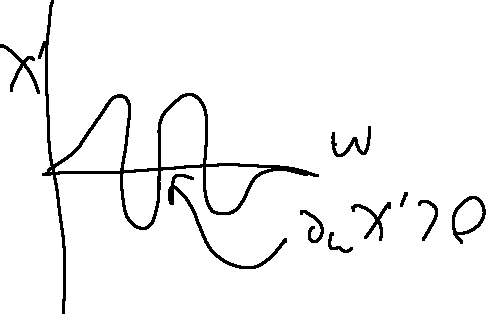
\includegraphics[width=10cm]{images/11-26-1.png}
	\caption*{Plot of 3LS $\chi'$}
\end{figure*}
Using this formula, when the slope becomes very high we will have light that has a group velocity much much slower than normal (as slow as 10m/s).
How do we understand this? We can think of this as the adiabatic passage of a dark state. If we start in the dark state, and send in a probe pulse then we will see our population remain in the dark state *which begins as $\ket{1}$.
\begin{figure*}[h!]
	\centering
	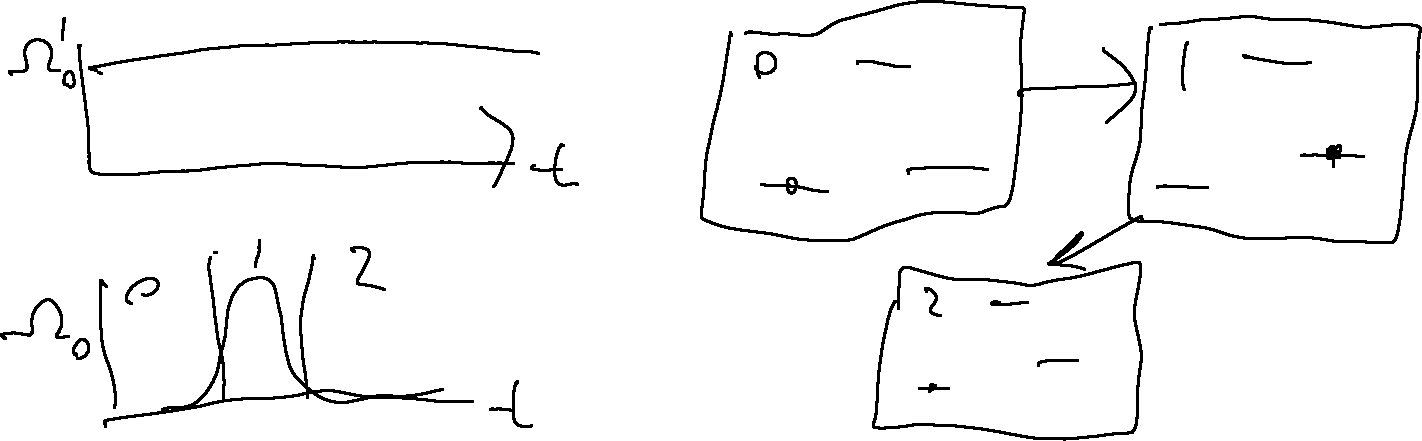
\includegraphics[width=10cm]{images/11-26-2.png} \\
	\caption*{Plot of the state as a pulsed probe is incident on the sample}
\end{figure*}
Once the probe arrives we see the population move to three, and then back to one as the pulse leaves.

Looking at the field we see this as an energy exchange. First we put energy from the field into the state for the transition from $\ket{1}\to\ket{3}$. Then we take energy out of the state and put it back into the field going from $\ket{3}\to\ket{1}$.
The rate of energy exchange is $~\Omega_0'$, so our group velocity scales with $\Omega_0'$. It can be shown that $v_g\propto\Omega_0'\ ^2$. This can be used to store light. If $\alpha L \gg 1$ then the probe is completely absorbed by the medium.
After this our $\rho_{13}$ is not zero. Not only not this value contains the information of the probe pulse. Therefore we say the probe pulse is stored in the medium as the coherence.

We want to know how to retrieve this information. In order to do this we simply need to apply a pump field to our sample.
\begin{figure*}[h!]
	\centering
	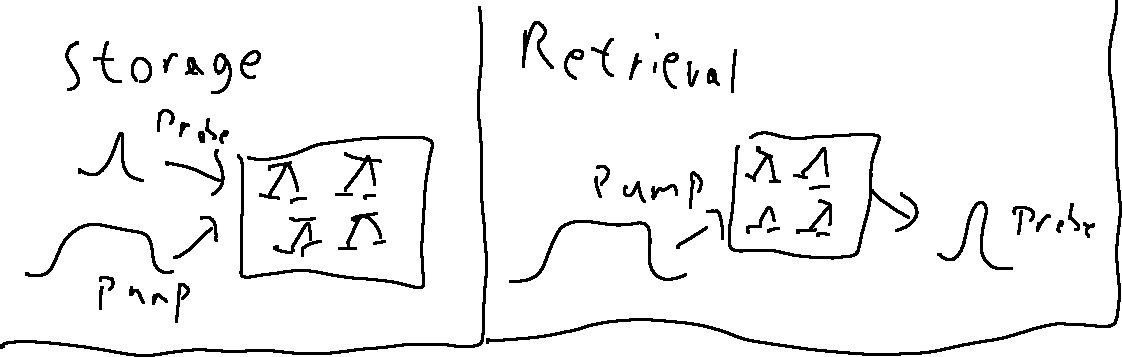
\includegraphics[width=10cm]{images/11-26-3.png}
	\caption*{Storage and retrieval of an optical field}
\end{figure*}
\subsection{Summary}
We introduced the idea of dark states, and used this idea to introduce the phenomena of coherent population trapping (related to $\rho_{22}$) and electromagnetically induced transparency (related to $\chi$).
Using adiabatic passage we also could see STIRAP, slow light and light storage. In all these our nonradiative coherence $\rho_{13}$ plays a central role.

Additionally we can see that for other types of three level systems (V or cascade). In both of these systems our $\rho_{13}$ decays via spontaneous emission, so it is shorter lived and these techniques aren't as powerful.
Finally we can look at EIT as a result of classical coupled harmonic oscilators.
\section{Mechanical effects of light}
\subsection{Overview}
The key insight of this section will be that light carries momentum (you can see this in Maxwell's equations).
In quantum mechanics we know that the momentum of a photon is $\hbar\bm{k}$. Therefore optical interactions must satisfy momentum conservation. The force applied is typcially quite small in macroscopic scales (~1W lasers will apply ~1nN of force).
Looking at the interaction of an atom with a photon instead, we see that not only will the atom's state change, but so will it's momentum, i.e. the change will be $\Delta\bm{p} = \hbar\bm{k}$, similarly for emission $\Delta\bm{p} = -\hbar\bm{k}$,
where in both of these $\bm{k}$ is the photon's wave vector.
\begin{figure*}[h!]
	\centering
	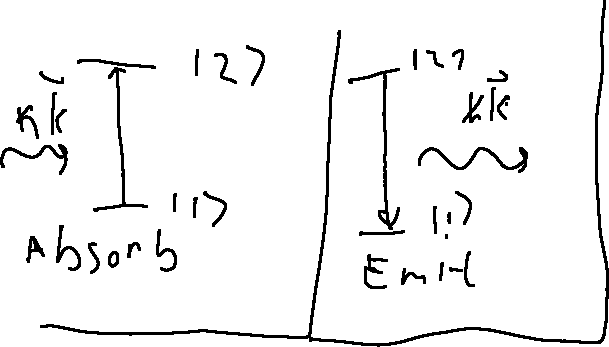
\includegraphics[width=10cm]{images/11-26-4.png}
	\caption*{Change in momentum from Emision and Absorption}
\end{figure*}
\subsection{Radiation Pressure}
This is sometimes called dissipative force. 

We start by ignoring spontatneous emission. This process will be absorption followed by stimulated emission, and since the wave vector will be the same for the absorbed and emitted light, then the overall change in momentum is zero.

\begin{figure*}[h!]
	\centering
	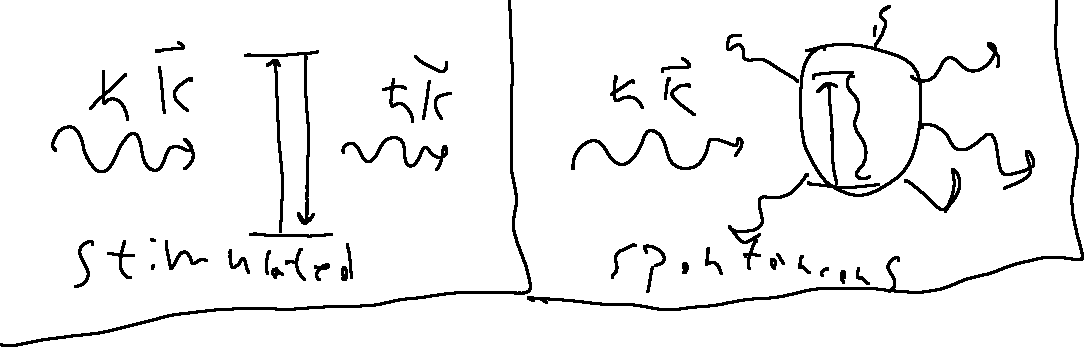
\includegraphics[width=10cm]{images/11-26-5.png}
	\caption*{Change in momentum from Stimulated and Spontaneous emission}
\end{figure*}

If we instead include the stimulated emission process, then we have $\hbar\bm{k}$ absorbed, and the $\hbar\bm{k}'$ emitted, where $\bm{k}'$ is the same magnitude as $\bm{k}$ but points in a random direction. On average the momentum change from the emission is zero,
therefore the total momentum change is going to be $\hbar\bm{k}$. If we continously shine a laser on a sample that will spontaneously emit photons, then the total change will be $\hbar\bm{k}\gamma_2\rho_{22}\Delta t$.
Therefore the force will be:
\begin{align*}
	\bm{F} &= \frac{\expval{\Delta \bm{p}}}{\Delta t} \\
	\bm{F} &= \hbar\bm{k}\gamma_2\rho_{22} \\
	\bm{F} &= \hbar\bm{k}\gamma_2\frac{\Omega_0|^2\gamma}{2\gamma_2}\frac{1}{\delta^2 + \gamma^2}
\end{align*}
And clearly the maximum force must be (because in steady state $\rho_{22} \leq \frac{1}{2}$):
\begin{align*}
	\bm{F}_\text{max} &= \frac{1}{2}\hbar\bm{k}\gamma_2
\end{align*}
\subsection{Doppler cooling}
We start by briefly reviewing the Doppler shift. If we look at an atom moving with a velocity $v$, we can say energy and momentum conservation together yield:
\begin{align*}
	m\bm{v} + \hbar\bm{k} &= m\bm{v}' \\
	\frac{1}{2}mv^2 + \hbar\omega_1 + \hbar \omega &= \hbar\omega_2 + \frac{1}{2}mv'\ ^2 \\
	\frac{1}{2}mv^2 + \hbar\omega_1 + \hbar \omega &= \hbar\omega_2 + \frac{1}{2m} (m\bm{v} + \hbar \bm{k})^2 \\
	\frac{1}{2}mv^2 + \hbar\omega_1 + \hbar \omega &= \hbar\omega_2 + \frac{1}{2}mv^2 +\frac{1}{2m} \hbar^2k^2 + \frac{1}{2}m\hbar\bm{v}\cdot\bm{k} \\
	\hbar\omega_1 + \hbar \omega &= \hbar\omega_2 +\frac{1}{2m} \hbar^2k^2 + \frac{1}{2}m\hbar\bm{v}\cdot\bm{k}
\end{align*}
Looking at $\frac{1}{2m} \hbar^2k^2$ we can see that this term will be very small, since $k$ is much smaller (when using equivalent units) than $m$, so:
\begin{align*}
	\omega_2 - \omega_1 &= \omega - \bm{k}\cdot\bm{v}
\end{align*}
So our resonance condition becomes $\omega_0 = \omega - \bm{k}\cdot\bm{v}$ where this shift to resonance is known as the Doppler shift.

If we choose our $\bm{k}$ along $\bm{v}$ then $\omega_0 = \omega - kv$, so the frequency of the light we send in is effectively down shifted (we need to use a higher frequency laser to drive the transition).

If instead we use $\bm{k}$ antiparallel to $\bm{v}$ then $\omega_0 = \omega + kv$, so the light we send in is effectively up shifted (we need a lower frequency laser to drive the transition).

\begin{figure*}[h!]
	\centering
	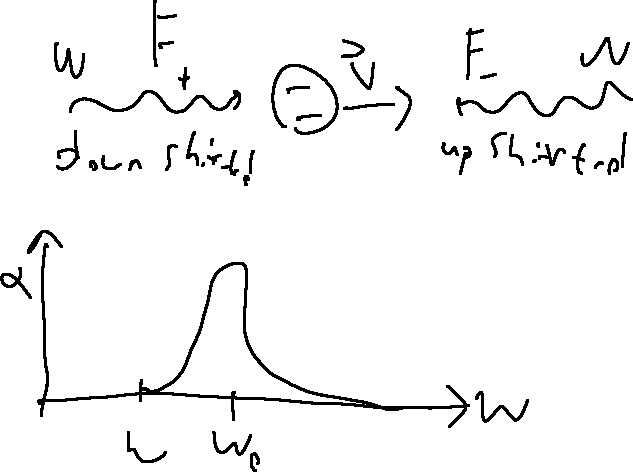
\includegraphics[width=10cm]{images/11-26-6.png}
	\caption*{Doppler cooling}
\end{figure*}
For doppler cooling we have two optical fields incident on an atom in opposite directions. By choosing $\omega$ less than $\omega_0$ we cause the force applied by the laser in the opposite direction of the motion to be greater than the one in the direction of motion.
This leads to a cooling/fricitional force/cooling force. We will eventually show $F\propto v$.

The exact (average) force we find for a moving particle is:
\begin{align*}
	F &= \frac{1}{2}\hbar k |\Omega_0|^2 \frac{\gamma}{(\omega_0 - \omega + \bm{k}\cdot\bm{v})^2 + \gamma'\ ^2}
\end{align*}
We now seek to calculate the net force applied by a our two lasers that are incident from different directiions:
\begin{align*}
	F_+ &= \frac{1}{2}\hbar k |\Omega_0|^2 \frac{\gamma}{(\omega_0 - \omega + kv)^2 + \gamma'\ ^2} \\
	F_- &= -\frac{1}{2}\hbar k |\Omega_0|^2 \frac{\gamma}{(\omega_0 - \omega - kv)^2 + \gamma'\ ^2}
\end{align*}
We now assume that the detuning is much greater than the doppler shift $|\omega - \omega_0| \gg kv$, so $(\omega_0 - \omega \pm kv)^2 \approx \delta^2 \pm 2\delta kv$. Therefore:
\begin{align*}
	F_\pm &= \pm\frac{1}{2}\hbar k |\Omega_0|^2 \frac{\gamma}{\delta^2 + \gamma'\ ^2}\frac{1}{1\pm \frac{2\delta kv}{\delta^2 + \gamma'\ ^2}} \\
	F_\pm &= \pm\frac{1}{2}\hbar k |\Omega_0|^2 \frac{\gamma}{\delta^2 + \gamma'\ ^2}\left(1\mp \frac{2\delta kv}{\delta^2 + \gamma'\ ^2}\right) \\
	F_\pm &= \pm F_0 - \frac{1}{2}\beta v
\end{align*}
Where:
\begin{align*}
	\beta &= 2\hbar k^2|\Omega_0|^2 \frac{\gamma}{(\delta^2 + \gamma'\ ^2)^2} \delta &
	F_0 &= \frac{1}{2}\hbar k |\Omega_0|^2 \frac{\gamma}{\delta^2 + \gamma'\ ^2}
\end{align*}
So our net force is then:
\begin{align*}
	F &= F_+ + F_- \\
	F &= -\beta v
\end{align*}
So we see we have a damping force. Additionally in practical experiments, as the atom cools, we would decrease the detuning to increase the effect of doppler cooling.

We now naturally wonder how cool can our Doppler cooling get. The key to understanding this is to understand what heating process counterbalances our cooling.
In fact the spontaneous emission process involves a random recoil, despite the fact it is our primary cooling process, it will also be our heating process.
In theremal equilibrium we know our heating and cooling rates will be equal. Our heating rate will be $\frac{(\hbar k)^2}{2M} \rho_{22}\gamma_2$, while the cooling rate is $\expval{\beta v^2}$. So in equilibrium:
\begin{align*}
	\frac{(\hbar k)^2}{2M} \rho_{22} \gamma_2 &= \expval{\beta v^2} \\
	\frac{(\hbar k)^2}{2M} \rho_{22} \gamma_2 &= \beta \frac{k_B T}{M} \\
	\frac{(\hbar k)^2}{2} \rho_{22} \gamma_2 &= \beta k_B T \\
	\frac{(\hbar k)^2}{2} \gamma_2 \frac{|\Omega_0|^2 \gamma}{\gamma_2(\delta^2 + \gamma'\ ^2)} &= k_B T 2\hbar k^2 \frac{|\Omega_0|^2 \gamma \delta}{(\delta^2 +\gamma'\ ^2)^2} \\
	k_B T &= \frac{\hbar}{4} \frac{\delta^2 + \gamma'\ ^2}{\delta} \\
	k_B T &= \frac{\hbar\gamma'}{2} \frac{\delta^2 + \gamma'\ ^2}{2|\delta|\gamma'}
\end{align*}
So:
\begin{align*}
	k_B T &> \frac{\hbar\gamma'}{2} \\
	T_D &= \frac{\hbar\gamma'}{2k_B}
\end{align*}
When first trying to verify this, experiments with $T_D \approx 170 \mu K$ yielded a temperature with $40 \mu K$! This was seen by multiple experiments, and took nearly a year to understand. The explination will be covered in the next lecture.

We already have a cooling force, but we also need to have a trapping force to keep the atoms in place. This can be done with a magneto optic trap.
\subsection{Another perspective}
We have so far looked at these mechanical effects from the perspective of momentum conservation. We ill now look at this from the perspective of dispersive, gradient and dipole forces. Starting from our interaction Hamiltonian:
\begin{align*}
	V &= -\bm{\mu}\cdot\bm{E} &
	\hat{\bm{F}} &= \partial_t \bm{p} \\
	\hat{\bm{F}} &= \frac{1}{i\hbar} [\bm{p}, V] &
	\hat{\bm{F}} &= -\del V
\end{align*}
So our average force is:
\begin{align*}
	\bm{F} &= \expval{\hat{\bm{F}}} \\
	\bm{F} &= -\expval{\del V}
\end{align*}
We now quickly express our potential explicitly:
\begin{align*}
	V &= \frac{\hbar}{2}\Omega_0\sigma_+ + \text{h.c.} &
	\sigma_+ &= \ket{2}\bra{1} \\
	\Omega_0(\bm{r}) &= -\frac{\mu E(\bm{r})}{\hbar} e^{i\phi(\bm{r})} & 
	\Omega_0(\bm{r}) &= |\Omega_0(\bm{r})|e^{i\phi(\bm{r})}
\end{align*}
So:
\begin{align*}
	F &= -\frac{\hbar}{2}\del \Omega_0\expval{\sigma_+} + \text{c.c.} \\
	\expval{\sigma_+} &= \rho_{12} \\
	\expval{\sigma_+} &= -\frac{\Omega_0^*}{2} \frac{1}{\delta + i\gamma} \frac{\delta^2 + \gamma^2}{\delta^2 + \gamma'\ ^2} \\
	\del \Omega_0 &= e^{i\phi}\del |\Omega_0| + i|\Omega_0| e^{i\phi} \del \phi \\
	\del \Omega_0 &= \Omega_0 \left(\frac{\del|\Omega_0|}{|\Omega_0|} + i\del\phi\right) \\
	\bm{F} &= \frac{\hbar}{4}|\Omega_0|^2 \frac{1}{\delta + i\gamma}\frac{\delta^2 + \gamma^2}{\delta^2 + \gamma'\ ^2} \left(\frac{\del|\Omega_0|}{|\Omega_0|} + i\del\phi\right) + \text{c.c.} \\
	\bm{F} &= \frac{\hbar}{4}|\Omega_0|^2 \frac{\delta^2 + \gamma^2}{\delta^2 + \gamma'\ ^2}\left(\frac{-i\gamma}{\delta^2 + \gamma^2} + \frac{\delta}{\delta^2 + \gamma^2}\right) \left(\frac{\del|\Omega_0|}{|\Omega_0|} + i\del\phi\right) + \text{c.c.} \\
	\bm{F} &= \frac{\hbar}{2}|\Omega_0|^2 \frac{\delta^2 + \gamma^2}{\delta^2 + \gamma'\ ^2}\left(\frac{\gamma}{\delta^2 + \gamma^2} \del\phi + \frac{\delta}{\delta^2 + \gamma^2} \frac{\del|\Omega_0|}{|\Omega_0|}\right) \\
	\bm{F} &= \frac{\hbar}{2}|\Omega_0|^2 \frac{1}{\delta^2 + \gamma'\ ^2}\left(\gamma\del\phi + \delta\frac{\del|\Omega_0|}{|\Omega_0|}\right)
\end{align*}
This force has two components, a dissipative force related to $\del\phi$ and a dispersive force related to $\del|\Omega_0|$.
\begin{align*}
	\bm{F}_\text{diss} &= \frac{\hbar}{2}|\Omega_0|^2 \frac{\gamma}{\delta^2 + \gamma'\ ^2}\del\phi \\
	\bm{F}_\text{disp} &= \frac{\hbar}{2}|\Omega_0|^2 \frac{\delta}{\delta^2 + \gamma'\ ^2}\frac{\del|\Omega_0|}{|\Omega_0|} \\
	\bm{F}_\text{disp} &= \frac{\hbar}{4} \frac{\delta}{\delta^2 + \gamma'\ ^2}\del |\Omega_0|^2
\end{align*}
We know for a plane wave $\del|\Omega_0| = 0$ and $\del\phi = \bm{k}$, so for a plane wave:
\begin{align*}
	\bm{F} &= \frac{\hbar}{2}\bm{k} |\Omega_0|^2 \frac{\gamma}{\delta^2 + \gamma'\ ^2}
\end{align*}
Which is what we derived before, so our dissipative force is the force we found for spontaneous emission/absorption.

If we work with a beam of spoot size $~a$, then we will have:
\begin{align*}
	\bm{F}_\text{disp} &\approx \frac{\hbar}{4} \frac{\delta}{\delta^2 + \gamma'\ ^2}\frac{|\Omega_0|^2}{a}
\end{align*}
If we instead look at writing our force in terms of a potential we can say that:
\begin{align*}
	\bm{F}_\text{disp} &= \frac{\hbar}{4} \frac{\delta}{\delta^2 + \gamma^2 + \frac{|\Omega_0|^2}{2}}\del |\Omega_0|^2 \\
	\bm{F}_\text{disp} &= - \del V_\text{opt} \\
	V_\text{opt} &= -\frac{\hbar\delta}{2}\ln \left(1 + \frac{1}{2}\frac{|\Omega_0|^2}{\delta^2 + \gamma^2}\right)
\end{align*}
If we are far off resonance, $\delta \gg \gamma_3$ and $\delta \gg \Omega_0$, then:
\begin{align*}
	V_\text{opt} &\approx -\frac{\hbar\delta}{2}\frac{1}{2}\frac{|\Omega_0|^2}{\delta^2} \\
	V_\text{opt} &\approx -\frac{\hbar}{4}\frac{|\Omega_0|^2}{\delta}
\end{align*}
Which is the optical stark shift. This can be used to create optical tweezers which hold particles in place using a spatially varying intensity.
Additionaly, this can be used to create an optical latice with a periodic potential, where atoms are trapped in one of many potential wells.
\begin{figure*}[h!]
	\centering
	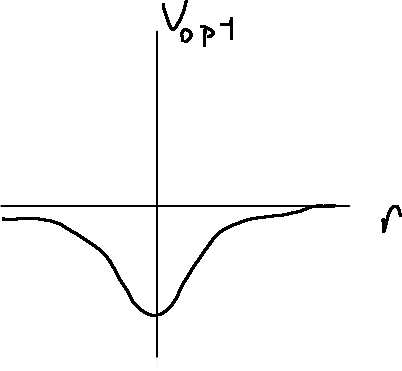
\includegraphics[width=10cm]{images/12-03-1.png}
	\caption*{Potential for Optical tweezers}
\end{figure*}
\begin{figure*}[h!]
	\centering
	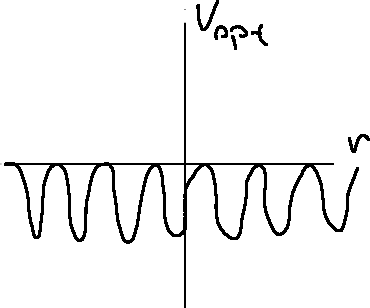
\includegraphics[width=10cm]{images/12-03-2.png}
	\caption*{Potential for Optical lattice}
\end{figure*}
Can we understand the optical stark shift now in terms of conservation of momentum? If our incoming wave is not a plane wave, then we have many wave vectors associated with our beam $\bm{k}$.
If we absorb and re-emit according to different $\bm{k}$s from our beam, then (after some math that is out of scope for what we are looking at), we will see the optical stark shift!

\subsection{Sub-Doppler cooling}
It is possible that the cooling below the doppler limit could be caused by a gradient force in the laser intensity.
Typically we expect to see our two laser fields with identical polarization, so they will form spatially standing waves.
If we make these polarizations orthogonal, there will be no spatial intensity modulation which surprisingly gives better results.
So this doesn't really seem to explain how we broke the doppler limit.

We next consider the additional energy levels of the atom, instead of looking at it as a two level system, we consider a hyperfinely split system (which has many energy levels).

We could also consider if there is a polarization gradient. If we have two conterporpogating fields with different polarizations then you find that the net polarization is circular:
\begin{align*}
	\bm{E}_l &= E_0\hat{e}_x e^{ikz} \\
	\bm{E}_r &= E_0\hat{e}_y e^{-ikz} \\
	\bm{E} &= \bm{E}_l + \bm{E}_r & \text{Assuming out of face for simplicity} \\
	\bm{E} &\propto (\hat{e}_x + i\hat{e}_y)\cos kz + i(\hat{e}_x - i\hat{e}_y)\sin kz \\
	\bm{E} &\propto \hat{e}_+\cos kz + i\hat{e}_y\sin kz
\end{align*}
Which are circularly polarized waves, with the portion of each polarization varying spatially. These two different polarizations cause our system to couple to multiple states.
The process of optical pumping then governs a dissipative process using these mechanisms.

To fully charactorize this process we would need to look at Clebsch-Gordon coefficients for different transitions, but instead here we approach this with a simplified model.
We consider in our model the $J=\frac{1}{2}\to J=\frac{1}{2}$ transition. 
\begin{figure*}[h!]
	\centering
	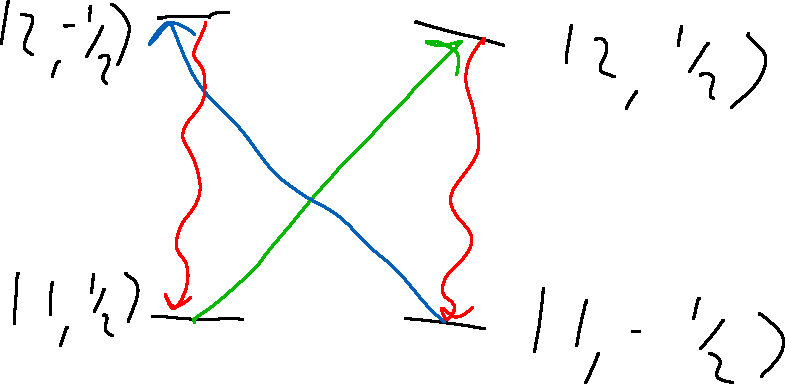
\includegraphics[width=10cm]{images/12-05-1.png}
	\caption*{Transitions for our model, in green is the $\sigma_+$ transition, in blue is the $\sigma_-$ transition and in red is the optical pumping transition}
\end{figure*}
As the atoms move around they reach the peak of their corresponding potentials due to the polarizations coopling to the other states.
At the peak they are most likely to be excited to a higher state, which then decays to a lower state that couples via the opposite polarization of light.
Therefore the atom finds itself at the bototom of a well, then they repeat this proces, losing $\frac{\hbar|\Omega_0|^2}{4|\delta|}$.
\begin{figure*}[h!]
	\centering
	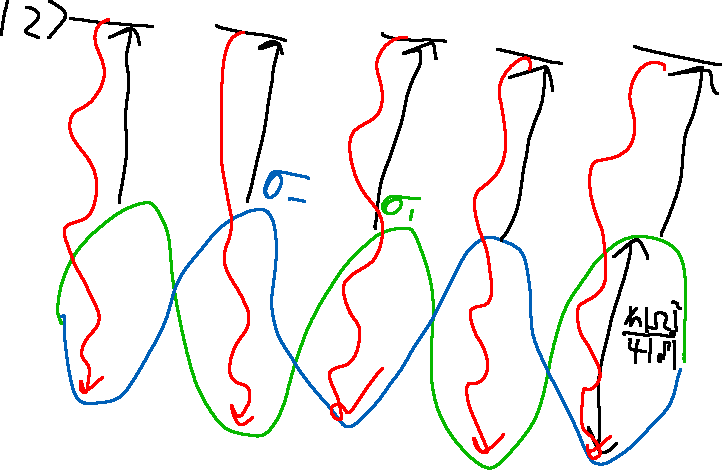
\includegraphics[width=10cm]{images/12-05-2.png}
	\caption*{Atoms in sysyphus cooling potential}
\end{figure*}
This process works well when $k_B T > \frac{\hbar |\Omega_0|^2}{4|\delta|}$. Additionally we have a recoil limit $\frac{(\hbar k)^2}{2M} = k_B T_r$.
This recoil limit is $T_R~1\mu K$.

Now we clearly want to concider how to circumvent this cooling limit. In order to do this we want to avoid spontaneous emission, and therefore avoid the excited state whenever possible.
In orer to avoid exciting the atom we utilize the dark state.

When we include the momentum in our state, we have the dark and bright states (when the fields are equal) are described by:
\begin{align*}
	\ket{D,p} &= \frac{1}{\sqrt{2}}(\ket{+1,p+\hbar k} - \ket{-1,p-\hbar k}) \\
	\ket{B,p} &= \frac{1}{\sqrt{2}}(\ket{+1,p+\hbar k} + \ket{-1,p-\hbar k})
\end{align*}
\begin{figure*}[h!]
	\centering
	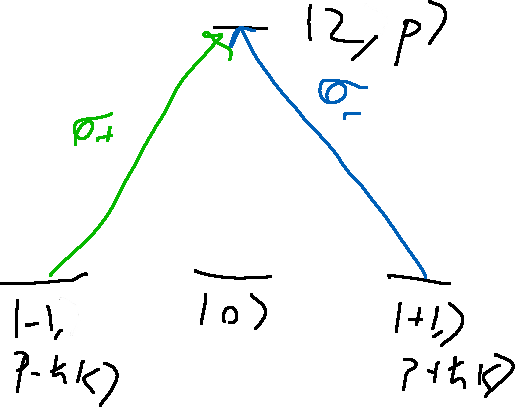
\includegraphics[width=10cm]{images/12-05-3.png}
	\caption*{Dark states in our sysyphus cooling setup}
\end{figure*}
We see that the $\ket{D,p}$ state is only dark if $p=0$. This allows for cooling because any state can be randomly put into $\ket{D,p}$ by random recoil, which will then stay in that state for all time since it is a dark state.
This is known as velocity selective CPT.

In trapped ions there is also the process of resolved sideband cooling.

\chapter{Winter Term, Brian Smith}
\section{Review}
\subsection{Classical Mechanics}
We can look at classical mechanics in terms of three different formalizims, all of these describe how classical particles move in space.

The first is the Newtonian model in which we describe things in terms of forces applied, i.e. $\sum\bm{F}  = m\ddot{\bm{x}}$.
As an example, take a particle moving with mass m in 1 dimension with an arbitrary potential, so:
\begin{align*}
	F &= -\partder{V}{x} \\
	m\ddot{x} &= -\partder{V}{x}
\end{align*}

The second is the Lagrangian formulation in which $L = T -V$, the equations of motion determined from $\delta S = 0$ where $S = \int L dt$. In other words this turns our problem into a variational calculus  problem.
\begin{align*}
	\delta S  &= \int \left(\partder{L}{q} \delta q + \partder{L}{\dot{q}} \delta \dot{q}\right) dt \\
	\delta S  &= \int \left(\partder{L}{q} \delta q - \frac{d}{dt}\partder{L}{\dot{q}} \delta q\right) dt \\
	\delta S  &= \int \left(\partder{L}{q}  - \frac{d}{dt}\partder{L}{\dot{q}}\right)\delta q dt \\
	\partial_q L &= \frac{d}{dt}\partder{L}{\dot{q}}
\end{align*}

As an example, take a particle moving with mass m in 1 dimension with an arbitrary potential, so:
\begin{align*}
	L &= \frac{m}{2}\dot{x}^2 - V(x) \\
	\partder{L}{x} &= -\partder{V}{x} \\
	\partder{L}{{\dot{x}}} &= m \dot{x} & \text{We call this term the conjugate momentum } p_x\\
	m \ddot{x} &= -\partder{V}{x}
\end{align*}
So here we see the result matches what we saw for Newtonian mechanics.

The third is the Hamiltonian formulation in which $H = \sum p_i \dot{q}_i - L$ (the legendre transform of the Lagrangian formulations). Here we first determine our conjugate momenta $p_j = \partder{L}{\dot{q}_j}$.
Then we construct $H = p_j \dot{q}_j - L$. Now we minimize the action again in terms of $q_j$ and $p_j$, but that is unweildy, so:
\begin{align*}
	\partder{H}{q} &= -\partder{q}{L} - \partder{L}{\dot{q}} \partder{\dot{q}}{q} + \partder{}{q} (p \dot{q}) \\
	\partder{H}{q} &= -\partder{q}{L} - \partder{L}{\dot{q}} \partder{\dot{q}}{q} + \partder{p}{q} \dot{q} + \partder{\dot{q}}{q} p \\
	\partder{H}{q} &= -\partder{q}{L} - \partder{L}{\dot{q}} \partder{\dot{q}}{q} + \partder{\dot{q}}{q} p \\
	\partder{H}{q} &= -\partder{L}{q} \\
	\partder{H}{q} &= -\dot{p}
\end{align*}
We now look at our other equation of motion:
\begin{align*}
	\partder{H}{p} &= \partder{}{p} (p\dot{q}) - \partder{L}{p} \\
	\partder{H}{p} &= \dot{q}
\end{align*}
Looking again at a particle with mass m in 1 dimension with an arbitrary potential:
\begin{align*}
	p &= m\dot{x} \\
	H &= p\dot{x} - L \\
	H &= \frac{p^2}{m} - \frac{p^2}{2m} + V(x) \\ 
	H &= \frac{p^2}{2m}  + V(x) \\
	\dot{x} &= \frac{p}{m} \\
	-\dot{p} &= \partder{V}{x} \\
	\ddot{x} &= \frac{\dot{p}}{m} \\
	m\ddot{x} &= -\partder{V}{x}
\end{align*}
Which again matches the Newtonian approach.

Alternatively we could use the Poisson formalism. We say the Poisson bracket is defined:
\begin{align*}
	\{f,g\} &= \sum_i \partder{f}{q_i}\partder{g}{p_i} - \partder{g}{q_i}\partder{f}{p_i}
\end{align*}

We can see that for any quantity:
\begin{align*}
	\{f,H\} &= \dot{f}
\end{align*}

If we now look at the motion of a pendulum:\\ 
\includegraphics*[width=8cm]{images/1-06-fig1.png} \\
We can quickly derive that:
\begin{align*}
	q &= l\theta \\
	V &= mgy \\
	p &= m\dot{\theta} \\
	\omega &= \frac{g}{q} \\
	H &= \frac{1}{2m} p^2 + \frac{m}{2} \omega q^2
\end{align*}

If we want to quantize a system we do two things: \\
0) Determine $H$, $p$ and $q$ for our classical system, such that the Hamilton equations of motion give correct classical dynamics. These must be canonically conjugate variables such that $p_i = \partder{L}{\dot{q}_i}$. \\
1) We then determine the Poisson brackets for $q_i$ and $p_i$. \\
2) We then change our canonically conjugate variables to operators acting on a Hilbert space, with commutators given by $[\hat{a},\hat{b}] = i\hbar\{a,b\}$

Now to quantize our pendulum:
\begin{align*}
	\hat{H} &= \frac{\hat{p}^2}{2m} + \frac{m\omega^2}{2}\hat{q}^2
\end{align*}
To solve this we use ladder/creation/raising/anihilation/lowering operators:
\begin{align*}
	\hat{a}^\dagger &= \sqrt{\frac{mw}{2\hbar}} \left(\hat{q} - \frac{i}{m\omega} \hat{p}\right) \\
	\hat{a} &= \sqrt{\frac{mw}{2\hbar}} \left(\hat{q} + \frac{i}{m\omega} \hat{p}\right)
\end{align*}
These operators are non-Hermition, and therefore they can't represent an observable. If we say we have energy eigenstates $\hat{H}\ket{\psi} = E\ket{\psi}$, we claim that $\hat{H}\hat{a}^\dagger \ket{\psi} = (E + \hbar\omega)\ket{\psi}$.
In order to show this we rewrite our Hamiltonian:
\begin{align*}
	\hat{q} &= \sqrt{\frac{2\hbar}{m\omega}} \frac{\hat{a} + \hat{a}^\dagger}{2} \\
	\hat{p} &= \sqrt{\frac{2\hbar}{m\omega}} m\omega\frac{\hat{a} - \hat{a}^\dagger}{2i}
\end{align*}

\section{Field Quantization}
There are two standard approaches to field quantization:\\\\
1) The standard approach (for high energy physics, Condensced matter theory (in which we would instead have an effective field theory)) involves writing down a Lagrangian density/Action in terms of a density:
\begin{align*}
	S &= \int dt L(\phi(\bm{x},t),\partial_\mu \phi(\bm{x},t),t) \\
	S &= \int dt d^3 x \mathcal{L}(\phi(\bm{x},t),\partial_\mu \phi(\bm{x},t),t)
\end{align*}
Which allows you to determine the equations of motion for classical fields. If you follow this procedure for a scalar field of mass $m$, then you end up finding a lagrange density:
\begin{align*}
	\mathcal{L} &= (\partial_\mu\phi)(\partial^\mu\phi) - m^2\phi^2 \\
	(-i\hbar\partial_t)^2\phi + c^2 (i\hbar\del)^2\phi &= m^2c^4\phi
\end{align*}
When we move towards a more complete theory of quantum mechanics, we realize that there are no particles, and rather all interactions are done by quantum fields, where the things we describe as particles are in fact excitations of quantum fields.
We will see that a photon is an excitation of the electromagnetic field that occupies a specific mode of the EM field.

Once we have our classical equations of motion here, we ``Raise'' fields and conjugate momenta into operators, and impose commutators:
\begin{align*}
	\hat{\phi}(\bm{x},t),&& \hat{\pi}(\bm{x},t) &= \partder{\mathcal{L}}{\dot{\phi}} \\
	[\hat{\phi}(\bm{x},t),\hat{\pi}(\bm{x}',t)] &= i\hbar\delta(\bm{x} - \bm{x}')
\end{align*}
(This is correct for scalar fields, and massive vector fields, but must be modified for spinor fields and massless vector fields)
\\\\
2) We will now start our approach with a review of classical Electromagnetism:
\subsection{Review of Classical Electromagnetism}
We start with Maxwell's equation:
\begin{align*}
	\del\cdot\bm{B} &=0 & \del\cdot\bm{E} &+ \frac{\rho}{\epsilon_0} \\
	\del\times\bm{B} &= \mu_0\bm{j} + \mu_0\epsilon_0\partial_t \bm{E} &
	\del\times\bm{E} &= - \partial_t \bm{E} \\
	\bm{H} &= \frac{1}{\mu_0} \bm{B} - \bm{M} &
	\bm{D} &= \epsilon_0\bm{E} + \bm{P}
\end{align*}
and the Lorentz force law:
\begin{align*}
	\bm{F} &= q(\bm{E} + \bm{v}\times\bm{B})
\end{align*}
We can define the Hamiltonian(energy for free fields) and the Lagrangian:
\begin{align*}
	H &= \int d^3x \frac{\epsilon_0}{2}\left[\bm{E}^2 + c^2\bm{B}^2\right] \\
	L &= \int d^3x \frac{\epsilon_0}{2}\left[\bm{E}^2 - c^2 \bm{B}^2\right]
\end{align*}
Where here we are looking at in vacua fields. We also have a pointing vector:
\begin{align*}
	\bm{S} &= \frac{1}{\mu_0}\bm{E}\cross\bm{B} \\
	\bm{P} &= \int d^3 x \bm{S} \\
	\bm{J} &= \frac{1}{\mu_0}\int d^3 x\bm{x} \cross (\bm{E}\cross\bm{B})
\end{align*}
Where $\bm{P}$ is linear momentum, and $\bm{J}$ is angular momentum. Finally we introduce scalar and vector potentials:
\begin{align*}
	\bm{B} &= \del\times\bm{A} \\
	\bm{E} &= -\del\phi - \partial_t \bm{A}
\end{align*}
These potentials imply:
\begin{align*}
	\del\cdot\bm{B} &= 0 &
	\del\cross\bm{E} &= -\partial_t \bm{B}
\end{align*}
These fields are invarient under the gauge transformation:
\begin{align*}
	\phi' &= \phi - \partial_t \chi \\
	\bm{A}' &= \bm{A} +\del\chi
\end{align*}
And commonly we choose to either use the Lorentz gauge:
\begin{align*}
	\del\cdot\bm{A} &= \frac{1}{c^2} \partial_t\phi
\end{align*}
Which lets us then construct $A_\mu = (\phi/c,\bm{A})$ and $\partial_\mu =(\partial_t/c,\del)$, so we can then say $\partial_\mu A^\mu$ is a Lorentz scalar. 

Or instead (which is the choice we will use in classical Electromagnetism) we can choose the Radiation or Coulomb Gauge:
\begin{align*}
	\del\cdot\bm{A} &= 0
\end{align*}
Which immediately implies:
\begin{align*}
	\phi(\bm{x},t) &= \frac{1}{4\pi\epsilon_0}\int d^3x' \frac{\rho(\bm{x}',t)}{|\bm{x} - \bm{x'}|}
\end{align*}
If we are in the free field ($\rho = 0$, $\bm{j} = 0$):
\begin{align*}
	\del\cdot\bm{E} &= \del\cdot(-\del\phi - \partial_t\bm{A}) \\
	\nabla^2\phi &= 0
\end{align*}
And:
\begin{align*}
	\del\times\bm{B} &= \del\cross\del\cross\bm{A} \\
	\del\times\bm{B} &= -\nabla^2\bm{A} \\
	(\nabla^2 -\frac{1}{c^2}\partial_t^2)\bm{A} &= 0
\end{align*}
So in the Coulomb gauge we see that the vector potential obeys the wave equation. Additionally $\bm{A}$ will be a transverse field, so the direction of propogation is perpendicular to the field itself.
Although this choice of gauge is not manifestly Lorentz invariant, i.e. the quantities change in different fields of reference, but we still see that our theory will obey relativity.
Additionally since in quantum optics we typically don't deal with frames that are related to eachother by relativistic speeds, we don't need to worry about maintaining exact Lorentz invariants here.

We now consider a free field in a cube of side $L$:

We start by expanding the classical EM field into a set of orthonormal modes. Where each individual mode is a solution to Maxwell's equations (in a particular geometry/ source configuration).
Here we choose to use plane waves as our modes, so:
\begin{align*}
	\bm{E} (\bm{x},t) &= \sum_{\bm{n}} \tilde{\bm{E}}_{\bm{n}}(t) e^{i\bm{k}_{\bm{n}}\cdot\bm{x}} + \compcon \\
	\bm{k}_{\bm{n}} &= (n_x,n_y,n_z) \frac{2\pi}{L}
\end{align*}
These are equivalent to imposing periodic boundry conditions on the edge of the box. For a general problem, we can take $L$ to $\infty$ to include the entire universe. Similarly we find:
\begin{align*}
	\bm{B}(\bm{x},t) &= \sum_{\bm{n}} \tilde{\bm{B}}_{\bm{n}}(t) e_{i\bm{k}_{\bm{n}} \cdot\bm{x}} + \compcon \\
	\bm{A}(\bm{x},t) &= \sum_{\bm{n}} \tilde{\bm{A}}_{\bm{n}}(t) e_{i\bm{k}_{\bm{n}} \cdot\bm{x}} + \compcon
\end{align*}
We can see that these must all be real valued fields, so $\tilde{\bm{E}}_{\bm{n}}^* = \tilde{\bm{E}}_{-\bm{n}}$, and also the same will be true for $\tilde{\bm{B}}_{\bm{n}}$ and $\tilde{\bm{A}}_{\bm{n}}$.

From:
\begin{align*}
	\del\cdot\bm{B} &= 0 &
	\del\cdot\bm{E} &= 0 &
	\del\cdot\bm{E} &= 0
\end{align*}
We know that:
\begin{align*}
	\del\cdot\bm{F} (\bm{x},t) &= \sum_{\bm{n}} \del\cdot\left((\tilde{\bm{F}}_{\bm{n}}(t) e^{i\bm{k}_{\bm{n}}\cdot\bm{x}} + \compcon\right) \\
	\del\cdot\bm{F} (\bm{x},t) &= \sum_{\bm{n}} i\bm{k}_{\bm{n}}\cdot\tilde{\bm{F}}_{\bm{n}}(t) e^{i\bm{k}_{\bm{n}}\cdot\bm{x}} + \compcon
\end{align*}
Which in order to hold for all choices of $\tilde{\bm{F}}_{\bm{n}}$ must imply:
\begin{align*}
	i\bm{k}_{\bm{n}}\cdot\tilde{\bm{F}}_{\bm{n}} &= 0 &
	\tilde{\bm{F}}_{\bm{n},s} &= \bm{\epsilon}_{\bm{n},s} E_{\bm{n},s}(t) \\
	\bm{\epsilon}_{\bm{n},s} \cdot\bm{k}_{\bm{n}} &= 0 &
	\bm{\epsilon}_{\bm{n},i}\cdot\bm{\epsilon}_{\bm{n},j}^* &= \delta_{ij}
\end{align*}

So we have:
\begin{align*}
	\bm{E}(\bm{x},t) &= \sum_{s=1,2}\sum_{\bm{n}} \tilde{E}_{\bm{n},s}(t) \bm{\epsilon}_{\bm{n},s} e^{i\bm{k}_{\bm{n}}\cdot\bm{x}} + \compcon
\end{align*}
And with our knowledge that $\del\times\bm{E} = -\partial_t\bm{B}$:
\begin{align*}
	i\bm{k}_{\bm{n}} \times \tilde{\bm{E}}_{\bm{n},s} &= (-\partial_t \tilde{\bm{B}}_{\bm{n},s}(t)) \bm{\beta}_{\bm{n},s} \\
\end{align*}
And with $\del\times\bm{B} = \frac{1}{c^2}\partial_t \bm{E}$, 
\begin{align*}
	(ik_{\bm{n}} \times\bm{\beta}_{\bm{n},s})\tilde{\bm{B}}_{\bm{n},s} &= \frac{1}{c^2} (\partial_t \tilde{\bm{E}}_{\bm{n},s}(t))\bm{\epsilon}_{\bm{n},s}
\end{align*}
And saying $l = (\bm{n},s), -l = (-\bm{n},s)$, and $\bm{k} = \bm{\mathcal{k}}_{\bm{n}} |\bm{k}_{\bm{n}}|$ so
\begin{align*}
	\bm{\mathcal{k}}_{\bm{n}} \times\bm{\epsilon}_l &= -\bm{\beta}_l &
	\bm{\mathcal{k}}_{\bm{n}} \times\bm{\beta}_l &= \bm{\epsilon}_l \\
	ik_{\bm{n}} \tilde{E}_l(t) &= \dot{\tilde{B}}_l(t) & 
	ik_{\bm{n}} \tilde{B}_l(t) &= \frac{\dot{\tilde{E}}_l}{c^2}
\end{align*}
From this we can see that we fixed our three basis vectors:
\begin{align*}
	\bm{\epsilon}_{\bm{n},1}\times\bm{\epsilon}_{\bm{n},2} &= \bm{\mathcal{k}}_{\bm{n}} \\
	\bm{\mathcal{k}}_{\bm{n}} \times\bm{\epsilon}_{\bm{n},1} &= \bm{\epsilon}_{\bm{n},2} \\
	\bm{\mathcal{k}}_{\bm{n}} \times\bm{\epsilon}_{\bm{n},2} &= -\bm{\epsilon}_{\bm{n},1}
\end{align*}
So we find:
\begin{align*}
	\bm{\beta}_{\bm{n},1} &= -\bm{\epsilon}_{\bm{n},2}
\end{align*}
And finally we see (recognizing that $k_l A_l = B_l$):
\begin{align*}
	\bm{E}(\bm{x},t) &= \sum_l \tilde{E}_l(t) \bm{\epsilon}_l e^{i\bm{k}_l\cdot\bm{x}} + \compcon \\
	\bm{B}(\bm{x},t) &= \sum_l \tilde{B}_l(t) (-i\bm{k}_l\times\bm{\epsilon}_l) e^{i\bm{k}_l\cdot\bm{x}} + \compcon \\
	\bm{A}(\bm{x},t) &= \sum_l \tilde{A}_l(t) \bm{\epsilon}_l e^{i\bm{k}_l\cdot\bm{x}} + \compcon
\end{align*}

Now we can apply the wave equation to any of our vector fields:
\begin{align*}
	\left(\nabla^2 - \frac{1}{c^2}\partial_t^2\right)\bm{F} &= 0 \\
	\left(-k_l^2 - \frac{1}{c^2}\partial_t^2\right)\tilde{A}_l(t) &= 0
\end{align*}
So:
\begin{align*}
	\tilde{A}_l(t) &= A_l e^{i\omega_l t} & \omega_l &= c k_l
\end{align*}
And finally:
\begin{align*}
	\bm{E}(\bm{x},t) &= \sum_l i\omega_lA_l \bm{\epsilon}_l e^{i(\bm{k}_l\cdot\bm{x} -\omega_l t)} + \compcon \\
	\bm{B}(\bm{x},t) &= \sum_l (i\bm{k}_l\times\bm{\epsilon}_l)A_l e^{i(\bm{k}_l\cdot\bm{x} - \omega_l t)} + \compcon \\
	\bm{A}(\bm{x},t) &= \sum_l \bm{\epsilon}_l A_l e^{i(\bm{k}_l\cdot\bm{x} -\omega_l t)} + \compcon
\end{align*}


\end{document}
